% \documentclass[format=acmsmall, natbib=false, review=false, authordraft=false, anonymous=true, screen=true]{acmart}
\RequirePackage{rotating}
\documentclass[format=acmsmall, natbib=false, anonymous=true, review=true]{acmart}

\usepackage{enumitem}
\usepackage{graphicx}  % another package that works for figures
\usepackage{epstopdf}
\usepackage{lscape}
\usepackage{wrapfig}
\usepackage{booktabs} % For formal tables
\usepackage{cleveref} % for better references
\usepackage{caption,subcaption}
\usepackage[english]{babel}% Recommended
\usepackage{csquotes}% Recommended
\usepackage[abbreviate=true, dateabbrev=true, natbib=true, isbn=false, doi=false, eprint=false, urldate=comp, url=false, maxbibnames=9, maxcitenames=2,  backref=false, backend=biber, style=ACM-Reference-Format]{biblatex}
\usepackage{siunitx}
\usepackage{tabularx}
\usepackage{xcolor}

\RequirePackage{rotating}

% % using biblatex
\let\citename\relax
% \RequirePackage[abbreviate=true, dateabbrev=true, natbib=true, isbn=false, doi=false, eprint=false, urldate=comp, url=false, maxbibnames=9, maxcitenames=2,  backref=false, backend=bibtex, style=ACM-Reference-Format,language=american]{biblatex}

% \addbibresource{reference.bib}
\addbibresource{hari.bib}
\renewcommand{\bibfont}{\Small}

%% author color
\newcommand{\hs}[1]{{\color{red}{#1}}}
\newcommand{\tc}[1]{{\color{blue}{#1}}}
\newcommand{\lwt}[1]{{\color{olive}{#1}}}
\newcommand{\kk}[1]{{\color{violet}{#1}}}

%% other packages
\usepackage[ruled]{algorithm2e} % For algorithms
\renewcommand{\algorithmcfname}{ALGORITHM}
\SetAlFnt{\small}
\SetAlCapFnt{\small}
\SetAlCapNameFnt{\small}
\SetAlCapHSkip{0pt}
\IncMargin{-\parindent}

%% Rights management information.  This information is sent to you
%% when you complete the rights form.  These commands have SAMPLE
%% values in them; it is your responsibility as an author to replace
%% the commands and values with those provided to you when you
%% complete the rights form.
\setcopyright{acmcopyright}
\copyrightyear{2021}
\acmYear{2021}
\acmDOI{10.1145/1122445.1122456}

%% These commands are for a PROCEEDINGS abstract or paper.
\acmConference[CSCW '21]{CSCW '21: The 24rd ACM Conference on Computer-Supported Cooperative Work and Social Computing}{Nov 03 -- 07, 2021}{Toronto, Canada}
\acmBooktitle{CSCW '21: The 24rd ACM Conference on Computer-Supported Cooperative Work and Social Computing,
Nov 03 -- 07, 2021, Toronto, Canada}
\acmPrice{15.00}
\acmISBN{978-1-4503-9999-9/18/06}


%%
%% Submission ID.
%% Use this when submitting an article to a sponsored event. You'll
%% receive a unique submission ID from the organizers
%% of the event, and this ID should be used as the parameter to this command.
\acmSubmissionID{123-A56-BU3}

%%
%% The majority of ACM publications use numbered citations and
%% references.  The command \citestyle{authoryear} switches to the
%% "author year" style.
%%
%% If you are preparing content for an event
%% sponsored by ACM SIGGRAPH, you must use the "author year" style of
%% citations and references.
%% Uncommenting
%% the next command will enable that style.
%%\citestyle{acmauthoryear}

%%
%% end of the preamble, start of the body of the document source.
\begin{document}

%%
%% The "title" command has an optional parameter,
%% allowing the author to define a "short title" to be used in page headers.
% \title[QV vs Likert]{``\textellipsis I can show what I really like.'': 
% Comparing Quadratic Voting with Likert Surveys at aligning respondents' preferences}

\title{``I can show what I really like.'': Eliciting Preferences via Quadratic Voting}


%%
%% The "author" command and its associated commands are used to define
%% the authors and their affiliations.
%% Of note is the shared affiliation of the first two authors, and the
%% "authornote" and "authornotemark" commands
%% used to denote shared contribution to the research.
\author{Ti-Chung Cheng}
\authornote{Both authors contributed equally to this research.}
\email{tcheng10@illinois.edu}
\affiliation{%
  \institution{University of Illinois at Urbana-Champaign}
}

\author{Tiffany Wenting Li}

\email{wenting7@illinois.edu}
\affiliation{%
  \institution{University of Illinois at Urbana-Champaign}
}

\author{Yi-Hong Chou}
\email{hank0982@link.cuhk.edu.hk}
\affiliation{%
  \institution{Independent Researcher}
}

\author{Karrie Karahalios}
\email{kkarahal@illinois.edu}
\affiliation{%
  \institution{University of Illinois at Urbana-Champaign}
}

\author{Hari Sundaram}
\email{hs1@illinois.edu}
\affiliation{%
  \institution{University of Illinois at Urbana-Champaign}
}

% %%
% %% By default, the full list of authors will be used in the page
% %% headers. Often, this list is too long, and will overlap
% %% other information printed in the page headers. This command allows
% %% the author to define a more concise list
% %% of authors' names for this purpose.
\renewcommand{\shortauthors}{Ti-Chung Cheng and Wenting Li, et al.}

%%
%% The abstract is a short summary of the work to be presented in the
%% article.
\begin{abstract}
  Decision-makers frequently aggregate self-reported data from the crowd to inform their decisions. One common case of collective decision-making involves prioritizing a subset of given options under resource constraints. Researchers have developed a wide range of surveying techniques,  such as ratings and rankings approaches, over the past century. However, it remains a challenge to eliciting accurate and rich self-reported responses in a resource-constrained context. In this study, we examine Quadratic Voting (QV), an alternative voting mechanism recently developed by \textcite{posner2018radical}, and argue that it could elicit self-reported responses more accurately compared to Likert scale when the survey goal is to understand relative preferences under resource constraints. We conducted two randomized controlled experiments on Amazon Mechanical Turk, one in the context of public opinion polling and the other in a human-computer interaction user study. Based on our Bayesian analysis results, a QV survey, with a sufficient amount of voice credits, aligned significantly closer to participants' incentive-compatible behaviors than a Likert scale survey, with a medium to high effect size. In addition, we extended QV's application scenario from typical public policy and education research to a problem setting familiar to the CSCW community: a prototypical HCI user study. Our experiment results, QV survey design, and QV interface serve as a stepping stone for HCI researchers to further explore this surveying methodology in their studies and encourage decision-makers from other fields to consider QV as a promising alternative.
%   While our study has shown QV's potential in obtaining more truthful self-reported relative preferences than Likert, the goal is not to claim that one survey instrument should replace another. Instead, we propose open questions about QV and encourage future research to consider promising alternative survey instruments that enhance self-reporting accuracy.
% Survey is a common approach to elicit individuals self-reported opinions in various fields. 
\end{abstract}

%%
%% The code below is generated by the tool at http://dl.acm.org/ccs.cfm.
%% Please copy and paste the code instead of the example below.
%%
\begin{CCSXML}
<ccs2012>
   <concept>
       <concept_id>10003120.10003130.10011762</concept_id>
       <concept_desc>Human-centered computing~Empirical studies in collaborative and social computing</concept_desc>
       <concept_significance>500</concept_significance>
       </concept>
   <concept>
       <concept_id>10003120.10003130.10003134</concept_id>
       <concept_desc>Human-centered computing~Collaborative and social computing design and evaluation methods</concept_desc>
       <concept_significance>500</concept_significance>
       </concept>
   <concept>
       <concept_id>10003120.10003121.10003122</concept_id>
       <concept_desc>Human-centered computing~HCI design and evaluation methods</concept_desc>
       <concept_significance>300</concept_significance>
       </concept>
 </ccs2012>
\end{CCSXML}

\ccsdesc[500]{Human-centered computing~Empirical studies in collaborative and social computing}
\ccsdesc[500]{Human-centered computing~Collaborative and social computing design and evaluation methods}
\ccsdesc[300]{Human-centered computing~HCI design and evaluation methods}

%%
%% Keywords. The author(s) should pick words that accurately describe
%% the work being presented. Separate the keywords with commas.
\keywords{Quadratic Voting, Likert scale, Empirical studies, Collective decision-making}


%%
%% This command processes the author and affiliation and title
%% information and builds the first part of the formatted document.
\maketitle
\section{Introduction}
Decision-makers often utilize surveys to aggregate opinions from the crowd to inform decisions. Understanding a crowd's preferences and priorities across a set of options under resource constraints is a common use case of surveys. \tc{When there are insufficient resources, such as money, time, space, and workforce, it is impossible to satisfy all the needs, creating a resource constraint scenario. Examples of these scenarios include public polling surveys designed to allocate government budgets \cite{pew_spending}, surveys to assess designs in human-computer interaction (HCI) interfaces \cite{ledo2018evaluation}, and surveys to prioritize what products to stock in grocery stores \cite{nielsen}.}

Likert scale is the current norm in many survey settings \cite{moors2016two}, including resource-constrained collective decision-making, because it is easy to administer and understand. For example, the Pew Research Center administered annual surveys with a 3-point Likert-like scale to \tc{know} how participants would budget federal government resources \cite{pew_spending}. In a Likert-like scale survey, participants can freely select ``increase spending'' for all government program areas without considering its feasibility under a limited government budget, a behavior known as the ``extreme responding'' bias \cite{batchelor2016extreme, furnham1986response, meisenberg2008acquiescent}. In this case, the inability to accurately elicit people's true preferences can lead to sub-optimal government budget allocation. Challenges with eliciting accurate self-reported preferences in resource-constrained decisions motivated us to examine an alternative, Quadratic Voting (QV), a relatively new voting mechanism proposed by \textcite{posner2018radical}. In this paper, we empirically tested how well QV elicits true preferences in resource-constrained collective decision-making processes compared to the Likert scale. \lwt{Here, we define an individual's ``true preference'' as a preference based entirely on their honest opinions and their own will.} \tc{We measure it through the outcome of an incentive-compatible task in our study.}

\tc{When making decisions under resource-constrained scenarios}, decision-makers ask the crowd two questions: (a) \textit{how much} do you prefer each option, and (b) how would you prioritize (i.e., rank) the options? Throughout the past century, researchers developed various forms of surveys to elicit true preferences via self-reporting. Ratings and rankings approaches are two of the primary categories in survey methods; they focus on answering one of the two questions above, but not both \cite{moors2016two}. 

% Ratings approaches, such as those used in Likert scales \cite{likert1932technique}, elicit attitude intensity to answer question (a), while ranking approaches that use a ranking scale \cite{starch1923methods}, ask question (b) \cite{moors2016two}. These limitations motivated us to examine an alternative that combines approaches from ratings and rankings, Quadratic Voting (QV), a relatively new voting mechanism proposed by \textcite{posner2018radical}. In this paper, we empirically tested how well QV elicits true preferences in resource-constrained collective decision-making processes compared to the Likert scale, the current norm in these processes \cite{moors2016two}.

% In order to find truthful answers, researchers have developed various forms of surveys to elicit \textit{truthful} self-reported preferences \cite{stone1999science}. 
% Rating and ranking-based surveys are the two major categories \cite{moors2016two}, each with their strengths and weaknesses. 

When responding to opinion-related questions in a rating-based survey, survey takers indicate their level of agreement, satisfaction, or importance along an intensity scale \cite{moors2016two}. The Likert scale is the most commonly used rating-based technique that elicits the \textit{strength} of a survey taker's preferences \cite{likert1932technique}. Rating-based surveys are easy to understand and administer; this may explain why the Likert scale is the current norm in many survey settings. In a resource-constrained scenario, however, a Likert scale survey may not accurately elicit how participants \textit{prioritize} \tc{the options since each option's statement is independent \cite{alwin1985measurement},} and a Likert scale survey does not safeguard against exaggerated or unrealistic preferences \cite{araujo2017much, vavreck2007exaggerated}.

On the contrary, ranking-based surveys focus on understanding how participants \textit{prioritize} the possible options \cite{moors2016two}, naturally incorporating the notion of resource constraints. For example, in participatory budgeting \cite{cabannes2004participatory}, a resource-constrained collective decision-making scenario where citizens vote for the projects that go into a government budget, participants use ranked voting to order the list of projects according to their relative preferences \cite{benade2020preference}. However, ranking-based surveys cannot elicit the \textit{strength} of a participant's preferences, i.e., how much more a participant values option A over B. Besides, performing statistical analysis on rankings data is challenging \cite{alwin1985measurement}.

There had been long debates on the pros and cons of rankings and ratings approaches. Nonetheless, when researchers developed many of these survey methodologies, the mediums of conducting surveys were paper and landlines. The current generation of survey tools, such as Survey Monkey and Qualtrics, simply translated the traditional approaches from paper to online. Given the ubiquity of personal computing devices today, such as \tc{smartphones, tablets,} and laptops, we ask: is there a computational-powered survey methodology that elicits both the rankings \textit{and} ratings of a set of options accurately in a resource-constrained collective decision-making process? In this study, we investigate Quadratic Voting (QV) \cite{posner2018radical} as a potential response to this question. 

Participants rank and rate the potential options in QV at the same time. In QV, expressing an opinion is not free -- each participant receives a fixed budget of voice credits, i.e., the ``currency" in QV, and pays a quadratic cost for the votes they cast. More formally, casting $n$ votes for or against an option costs $n^2$ voice credits. Participants vary the number of votes to represent the strength of their preference, i.e., they \textit{rate} an option with the number of votes. But as the number of votes on an option increases, the marginal cost for each extra vote increases as well; in other words, each additional vote becomes more expensive. Participants may cast as many votes as they choose on any option, as long as the total cost for the votes does not exceed the fixed given budget of voice credits. The limited budget and increasing marginal cost \tc{encourage} participants to make trade-offs among options, equivalent to \textit{ranking} them. Prior work further demonstrated that QV outcomes approximated a normal distribution\tc{ instead of }the polarized responses from Likert scale survey results on highly-debated topics \cite{quarfoot2017quadratic}. However, to the best of our knowledge, no one has empirically explored whether QV \tc{can elicit} more accurate self-reported preferences.
%\textcite{lalley2018quadratic} proved that the QV mechanism is more Pareto-optimal than many traditional voting mechanisms.

In our study, we examined QV's ability to elicit true preferences in resource-constrained collective decision-making processes. Given that Likert scale surveys are the most widely adopted to date \cite{moors2016two}, we compared a QV survey to a Likert scale survey \cite{likert1932technique} in a resource-constrained setting. We identified two distinct types of survey questions in this setting: (1) choosing among $K$ independent options of one topic, and (2) choosing among $K$ dependent options that jointly contribute to the same topic. To offer an analogy, scenario one relates to choosing among ice cream, cakes, and puddings for dessert, while scenario two assesses what an individual cares more about when choosing ice cream -- the flavor, texture, or ingredients. Therefore, we analyzed them in two separate research questions:


\begin{itemize}
    \item[\textbf{RQ 1}] How do QV responses align with people's true preferences compared to Likert scale responses in a survey where survey respondents choose among $K$ independent options of one topic? How do variations in the number of voice credits given to QV survey respondents impact this outcome?

    \item[\textbf{RQ 2}] How do QV responses align with people's true preferences compared to Likert scale responses in a survey where survey respondents choose among $K$ dependent options that jointly contribute to the same topic? 
\end{itemize}

To answer RQ1, we designed a public polling survey to assess which social causes need more support, a typical scenario for choosing among $K$ independent options. To measure participants' true preferences on the same topic, we created an incentive-compatible donation task, in which participants should only donate more for cause A than cause B if they truly care more about cause A \cite{champ1997using}. Participants on Mechanical Turk (MTurk) completed either a 5-point Likert scale version or a QV version of the survey, and the donation task, in a randomized controlled experiment. \tc{Since we were not aware of any prior work that empirically explored a way to determine the voice credit budget of QV, we asked the second question in RQ1. We experimented with} three variations of the QV survey with a small ($O(K)$), medium ($O(K^{1.5})$), and large ($O(K^2)$) budget in the experiment. We measured the similarity between each individual's survey result and their true preferences as reflected in the donation task and applied Bayesian analysis to compare the degree of similarity to true preferences in QV and Likert scale surveys.

In the case of choosing among $K$ dependent options that jointly contribute to the same topic in RQ2, we used an HCI user study scenario to understand how users make trade-offs across visual and audio elements in a video streaming experience given limited internet bandwidth. We used QV and 5-point Likert scale surveys to obtain participants' self-reported responses and designed \tc{an} incentive-compatible product design and pricing task to elicit their willingness-to-pay for each video element \cite{roth1982incentive}. Similar to the first experiment, we conducted the randomized controlled experiment on MTurk and analyzed the results with Bayesian analysis.

\textbf{Contributions} This work contributes to the extensive body of work on survey techniques that elicit self-reported preferences in resource-constrained decision-making in two ways: we find an improved accuracy of responses via QV compared to the Likert scale norm, and we extend the use of QV to the HCI user study domain.

\begin{description}
\item[QV elicits true preferences more accurately:] We show empirically that QV with a medium (i.e., $O(K^{1.5})$) to large (i.e., $O(K^{2})$) voice credit budget elicits true preferences more accurately than Likert scale responses when the survey respondents are asked to either (1) choose among $K$ independent options of the same topic, or (2) choose among $K$ dependent options jointly contributing to the same topic, under resource constraints. \tc{Unlike} prior empirical work that compared the characteristics of QV and Likert scale responses \cite{quarfoot2017quadratic, naylor2017first}, we focus on accurate preference elicitation. Based on two carefully-designed randomized controlled experiments, our Bayesian analysis showed that QV responses aligned significantly closer to participants' responses in an incentive-compatible task \tc{than the} 5-point Likert scale responses with a medium to high effect size. This finding is important because it shows that QV, a computational-powered alternative survey approach that combines ratings and rankings, \tc{can} assist resource-constrained decision-making with more accurate self-reported responses.
\item[Application of QV to HCI:] We extend QV's application scenario from typical public policy and education research to a problem setting familiar to the CSCW community: a prototypical HCI user study. The limited empirical studies and applications of QV focused mostly on public policy \cite{quarfoot2017quadratic, colorado_qv} and education research \cite{naylor2017first}. To the best of our knowledge, no HCI study has applied QV in a survey before. We designed an HCI user study with a research question that involved resource-constrained decisions and showed that a QV survey \tc{could} elicit users' preferences on an HCI-related research question more accurately than a Likert scale survey, a norm in the HCI community \cite{ledo2018evaluation}. Our experiment results, QV survey design, and QV interface serve as a stepping stone for HCI researchers to further explore the use of this surveying method in their studies and encourage decision-makers from other fields to consider QV as a promising alternative.
\end{description}

While our study demonstrates the potential of QV as a computational tool to facilitate truthful preference elicitation, the goal of this research is \textit{not} to convince decision-makers to replace their Likert scale surveys with QV surveys entirely. Indeed, in cases including when the survey requires the use of \tc{paper-based} responses (e.g., when technological aids are unavailable) or when the survey involves a list of unrelated options, QV may not be an appropriate option. Instead, our goal with this paper is to show that in the ratings and rankings scenarios that we investigate in this paper, QV may prove to be a compelling alternative to \tc{the} Likert scale when conducting online surveys.  

% we pose many open questions to prompt further conversations in the community, and encourage decision-makers to carefully evaluate QV's strengths and weaknesses (e.g., higher cognitive cost, less known to participants) prior to adoption.
% accuracy


% wider application domains



% ask participants to express their attitudes using a scale for a given topic or question on a scale of 1 to 5. Researchers would use collected responses to make their decision. This paper focuses on collective decision-making tasks aimed at eliciting group preferences among a set of choices among $K$ options. Questions such as: ``Which interface do users like most?'', ``What are some products that customers are satisfied with?'', and  ``What public policies do constituents feel more important?'' are examples of eliciting group preferences among $K$ options.


% \textit{RQ1.} How do results from QV, Likert survey align with people's incentive-compatible behavior when surveying societal issues? 

% We designed an experiment to compare how participants donate with QV and Likert survey results. We analyzed data using Bayesian analysis and qualitative analysis. We hypothesized that QV results better portray individuals' true beliefs as reflected by their monetary donations.

% \textit{RQ2.} How do results from QV and Likert-scale align with people's incentive-compatible behavior with a choice of HCI research questions? 
% To the best of our knowledge, no HCI studies used QV in their studies. Similar to the first experiment, we compare results from QV and Likert surveys with participant's behaviors in a video-element HCI experiment. We hypothesize that QV more accurately reflects the intensity of individuals' true beliefs. 

% \textit{RQ3.} How do different quantities of voice credits impact the results of QV empirically?
% We did not find studies on how many voice credits a participant should receive for QV in related literature. In conjunction with RQ1, we provide participants with a different number of voice credits. We suspect different outcomes from QV when participants have a different number of voice credits.


% is prone to reduced data quality. 
% Since each statement of Likert survey is independent when answering, \textcite{alwin1985measurement} found participants respond with the first acceptable answer instead of compiling an optimal solution. Another fallacy follows similar logic where participants would express opinions to the extreme, exaggerating one's actual belief \cite{araujo2017much, vavreck2007exaggerated}. This is due to Likert survey's nature of not incorporating the notion of resource constraints in the real word where it actually exists, for example, in the case of allocating budget for government spending. Participants in the example could express having large budgets for all causes, which in reality, in not possible because the budget is limited. Some researchers tried to introduce constraints to rating based surveys, for instance knapsack voting, developed by \textcite{goel2015knapsack}, forces participants to elect agreement only if the sum of the cost for the selected items is less than a given budget.

% For example, ranking scales is a ranking-based technique created by \textcite{starch1923methods} in 1923. Participants ranks a list of options in the order of their preferences in a ranking scale survey. Though researchers believe ranking demonstrated better reflects individuals' accordance, they are harder to statistically analysis and more cognitive demanding to participants \cite{moors2016two}. In other words, people are forced to make distinctions between options for rank-based surveys and applying constraints, i.e., there can only be one item ranked first. When taking budget into considerations, researchers developed value-for-money-ranking which asks participants to rank according to not just how they value the options, but the value-cost ration of the options. The biggest drawback of rank-based methods is giving up the information of \textit{strength} among their standings, i.e., how far apart is the first preference compared with the second? 


% Since early 1980s when investigators start to distribute surveys using internet-connected devices, electronic-mediated surveys merely translate paper-based surveys onto a webpage. Researchers did not make noticeable changes on the \textit{survey mechanisms} that unleashes the power of computation. Given the computing power of computers today and the omnipresence of computers at any individual's hands, can a better surveying mechanism harness computational advantages to obtain more accurate survey results?

% In this paper, we examine an alternative, Quadratic Voting (QV), a relatively new voting mechanism proposed by \textcite{posner2018radical}, to elicit more truthful self-reported responses in resource-constrained collective decision making processes. 

% Distribution of surveys for resource-constrained decision making is pervasive in everyday life and these surveys have been effective at aggregating people's attitudes to form consensus. Think tanks design and deploy large-scale ordinal scale polls \cite{pew} to understand public opinions on government policies given limited government resources. Supermarkets collect individuals' shopping experiences across products because there are limited shelves \cite{nielsen}. 

%% electronic decision making surveys merely transform from paper, but hasn't done much extra with the computational power; 
% Before the 1980s, research surveys required large-scale in-person participation. Slowly, surveys evolved into mail-in, telephone, and, eventually, online formats. In the early 1980s, researchers introduced electronic surveys to individuals as internet-connected devices became accessible. \kk{How did people take these? Not too many people had ISP service in the 80s. Which companies administered them?} They are limited to international companies and fortune 500 in 1985. Electronic surveys aimed to reduce research costs, reduce human labor required to conducted surveys, and add additional flexibility in survey design\cite{kiesler1986response}. While the \textit{medium} of how researchers conducted the surveys moved from offline to online, researchers did not make noticeable changes on the \textit{survey mechanisms} that unleashes the power of computation. We argue that electronic-mediated surveys merely translate paper-based surveys onto a webpage. Given the computing power of computers today and the omnipresence of computers at any individual's hands, can a better surveying mechanism harness computational advantages to obtain more accurate survey results?

% QV is an example of utilizing the computational power, and have xxx, xxx, xxx proven benefits in previous work; 

% In this study, , given that quadratic computations are difficult to conduct on paper or verbally due to the required cognitive load.

% we also want to confirm if QV is "accurate" enough in soliciting people's opinions
% Since Likert is the most commonly used form of a survey; we compare QV's accuracy with Likert's; 
% Since surveys are deployed to accurately understand people's attitudes, this paper aims to understand how how well QV survey results align with real world behaviors and beliefs?. To the best of our knowledge, there have not been any empirical studies that investigated to what degree does QV results align with participants' underlying true preferences. 


%Self reported data, that is data supplied by the survey participant is at the core of such surveys across a wide range of disciplines, from medicine to social services \cite{stone1999science}. To address this, researchers, have designed different types of survey mechanisms throughout the past century. In 1923, 
%In another survey approach, pairwise preference, developed by \textcite{scheffe1952analysis} in 1952, participants compared two choices by stating their preferences in one of seven intensity levels. Researchers developed these methods to better elicit individual attitudes under different settings and for different goals. Many of the proposed methods, however, fail in capturing authentic signals due to self-reporting bias or <define it>.
% how to use a survey and when to use it is also important
%

% This paper offers three major contributions.
% First, we designed two empirical studies and found that QV aligns better with the participant's underlying preferences when surveying people's preferences among $K$ options. The first experiment looked at eliciting societal causes while the other experiment pertains to HCI. Both of these experiments used participant behaviors as a baseline to measure these differences, which we argue is much stronger than the direct comparison to Likert that prior studies lean on. The results allowed us to argue that researchers should harness computers' power to utilize and benefit from deploying QV in studies if the study aims to understand people's preferences among $K$ options.

% Second, we demonstrate that QV results depend on the voice credit budget. To the best of our knowledge, little did researchers discussed the effect of the number of voice credits in prior works. In this study, we discovered that participants need a large enough voice credit to obtain an accurate QV result.

% The third contribution demonstrates the application of QV in the HCI domain. We are not aware of prior studies in HCI that utilize QV, and we believe that our experiment and software deliverable provides a template to use QV in later research.












%%----------------------------%%




% understanding how to apply QV in real-world scenarios, what challenges QV might face, and design decisions that can influence QV participants.

% \textbf{Design Implication}
% TODO. Talk about interface, future work and insights.


% Our first question focused on whether QV consistently produces a different result from the Likert survey results in an HCI study. Although usually applied to surveys in the social sciences, we hypothesize that QV could produce a cleaner and more accurate result than a Likert survey in an alternative setting such as Human-Computer Interaction (HCI). We designed one pretest experiment and one follow-up experiment to verify our hypothesis. In the pretest, we replicated the study developed by Quarfoot et al. \cite{quarfoot2017quadratic} and swapped the content of the survey with an HCI security study by Leon et al. \cite{leon2013matters} to show that QV extracts more fine-grain information compared to Likert. Results from the pretest aligned with the results by Quarfoot et al., suggesting that QV works under scenarios outside of societal-focused settings. 

%%%%%%%% old text from thesis
% Commercial companies deploy online surveys to understand which improvements users would like to see prioritized for a similar constraint. 
% Other surveys can be found in shopping centers to . 
% Data scientists and product teams also use surveys for them to prioritize mission-critical issues that customers face when deploying a product upgrade. 
% All these examples demonstrate how prevalent groups and institutions used surveys to make decisions by gathering consensus from surveying individual's attitudes.
% Our second question regards how QV and Likert-scale align with an individual's preferences expressed via their behavior across societal issues. We carefully redesigned a new experiment involving a larger group of participants to compare the alignment of QV and Likert surveys with a person's actual behavior. In this experiment, participants expressed their attitudes across societal causes and were given the option to donate to charitable organizations associated with each cause. We took a Bayesian approach to analyze the statistical power and effect size of how closely the Likert Survey and QV align with one's donation distribution. The results found statistical evidence that QV outperforms Likert if there are enough voice credits. Our third question looked at whether a different number of voice credit budget impacts people's voting behavior in QV. We used both experiments, the pretest experiment, and the formal experiment to test this idea. We found through qualitative and quantitative analysis that QV surveys require a significant amount of voice credits. We describe these research question more thoroughly in Chapter \ref{RQ}.

% Since then, this surveying method has been fully adopted by researchers and marketers alike. 
% Some researchers attributed this to the survey's ease of use. However, this ease of use does not guarantee the ease of analysis. Researchers today easily misuse Likert surveys by applying the incorrect analysis methods \cite{bishop2015use} or misinterpreting the analysis results \cite{jamieson2004likert, pell2005use}, leading to doubtful findings. Examples of such includes calculating the mean and standard deviations to interpret the data collected through a Likert survey. Even when applied correctly, there is usually little justification for using Likert surveys over other research tools in their research. 

% and how well it aligns with other surveying methods such as Likert survey. Further, we did not find any empirical study examining whether a different amount of voice credits impacts QV's result.
% Researchers have compared the Likert survey with QV from empirical and theoretical perspectives \cite{quarfoot2017quadratic, naylor2017first}. Cavaille et al. argued that QV outperforms Likert surveys among a set of political and economic issues \cite{cavaille2018towards}. 

% Surveys have been a useful tool at aggregating 
% Research agencies, industry labs, or independent researchers often hope to understand how to allocate resources better or to address people's preferences more accurately. 
% Agencies collect these surveys of huge crowds as a form of collective decision making. 


%%%%%%% old text from QV draft
% Likert survey is one of the most widely used methods to obtain the participant's opinion in the realm of human-computer interaction. Survey participants would express a rating across a series of measurements --- \textit{Very agree to very disagree} or \textit{On a scale of 1 to 5} --- for a listed statement. Very often, these opinions help researchers or decision-makers uncover consensus  across a group of people. However, there had been findings of how researchers can easily misuse Likert surveys either applying incorrect analysis methods  \cite{bishop2015use} or misinterpreting the analysis results \cite{jamieson2004likert, pell2005use} leading to questionable findings.In addition,  many research papers do not explain the rational behind the use of  Likert surveys. In a community that adopted Likert surveys almost as the defacto standard, we ask a fundamental question: ``Is Likert-scale survey the ideal method to measure collective attitudes for decision making?''
% Research agencies, industry labs or independent researchers often want to understand how to better allocate resources or what to improve upon. This is an example of eliciting user preferences  among $K$ options. These opinions are collected among huge crowds, as a form of collective decision making. For example,  ordinal scale polls were designed to understand public opinions on government policy \cite{pew} because there is limited funding. Companies deploy online surveys  to understand how product users  feel about the features and services that needs further improvements because companies have limited time  to develop the next release. Physical surveys can be found  in shopping centers to collect an individual's experiences for products on the shelf because there are limited shelves. All these examples demonstrated how surveys are often tied to  making decisions  by gathering consensus from surveying individual's attitudes. 
% In this study, we look at an alternative method called Quadratic Voting (QV). Published in 2015, \textcite{posner2018radical} proposed Quadratic voting as a voting mechanism with approximate Pareto efficiency.Under this voting mechanism,voters were initially given a fixed amount of voice credits (VC).With the credits, individuals can purchase any number of votes to support any of the statementslisted on the ballot. However, the cost of each vote increases quadratically when voted toward the same option.The authors proved that this mechanism is more efficient at making a collective decision because it minimizes welfare loss.Since 2015, a few studiescompared Likert surveys with QV empirically and theoretically\cite{quarfoot2017quadratic, naylor2017first}.\textcite{cavaille2018towards} argues that QV reflects one's opinion better compared to Likert-scale surveys when surveying one's opinionamong a set of political and economic issues.Despite these findings,we are not aware of related works thatcompare Likert surveys and QVwith participants' underlying true preferences.Therefore, it is unclear whether or notand in what degreedoes QV results align with participants' behaviors.In addition, no current work, to the best of our knowledge,deployed QV in the area of HCI.
%\end{enumerate}
% To answer these research questions,
% we designed two experiments.
% The first experiment,
% designed to answer RQ1 and RQ3,
% is a between-subject study
% where participants express their attitudes
% among a set of societal causes using 
% QV and Likert surveys
% and then donate
% to organizations relevant to these organizations.
% The second experiment 
% created an HCI study environment,
% aimed to answer RQ2,
% where participants were asked about 
% opinions among different video elements
% and their opinions using QV and Likert surveys.
% Our results showed that both experiments support
% QV in providing a clean and efficient way
% compared to Likert surveys
% at eliciting participant's true preferences.

\section{Related Works} \label{related_works}
In this section, 
we present related works
that discussed the challenges
of Likert survey
and related works of QV.

\subsection{Likert Scale Surveys}
Likert surveys are commonly deployed
to collects participant's opinions
because of its ease of use.
These surveys are deployed
to validate findings or clarify hypotheses
\cite{ozok2009survey, ledo2018evaluation} in HCI.
They are also used to verify or uncover the user's needs.
Likert surveys were invented by \textcite{likert1932technique} 
in \citeyear{likert1932technique},
which utilized a scale to deploy step-intervals 
from one attitude to the next.
Researchers today design 3, 5, 7, 
or even 12-point Likert surveys to accommodate different uses
\cite{garland2008computer,finstad2010}.
In addition, these surveys
can ause verbal descriptions
to segment the intervals,
presenting the choices with an ordinal scale.
Some researchers looked at
alternative presentations of the Likert scale
such as slider scales \cite{roster2015exploring} 
or phrase completions \cite{hodge2003phrase}, 
which aimed to circumvent 
some of the shortcomings of the traditional Likert scale.

There are, however, widespread controversies in the community on
when, why, and how to use Likert surveys \cite{bishop2015use}.
For instance, 
researchers sometimes misuse statistical method,
such as using mean and standard deviations \cite{jamieson2004likert},
to understand outcomes
when working with an ordinal metric.
Quantifying aggregated ordinal scale Likert surveys,
such as an average of ``1.5 agree'' can be unclear,
given that there does not exist ``agree and a half''
in real life.
Besides, 
options on the Likert scale can be stepwised.
One should not assume scale intervals to be equal.
In other words,
the difference between
``strongly agree'' and ``agree'' can be different 
when compared to the difference between
``neutral'' and ``agree'' \cite{jamieson2004likert, edmondson2005likert}.

An empirical study by \textcite{quarfoot2017quadratic}
identified another challenge
where people exaggerate their views
when filling out political surveys.
In this study,
participants often express polarized opinions
or have no opinion at all,
making it hard to form optimal conclusions \cite{posner2018radical}.
% When the results were aggregated, 
% a ``W'' shape distribution.
%This distribution demonstrated how people stand upon polarized views,
This occurrence was 
theoretically proved by \textcite{cavaille2018towards},
where respondents tend to overstate their values
if they want to influence the results through the survey.
These challenges motivated us 
to understand whether QV can fill the gap of inaccuracy
and provide a more accurate measurement
for collective decision making.\par

\subsection{Quadratic Voting}
Voting is often excercised
for collective decision making.
Quadratic voting originated 
from the argument
that current one-person-one-vote (1p1v) system
can easily bias toward the majority's opinion
and omitting the minority's votes.
This phenomenon is termed as 
the ``Tyranny of the Majority''
which criticizes that democratic decision
can easilty neglect those in need 
\cite{posner2018radical}.
In addition, 1p1v suffers the inability
for individuals to express fine-grain opinions
on the options one voted \cite{sep-voting-methods}.
Ranked-based voting tried to resolve this
by allowing voters to rank the options.
This mechanism can
suffer from Condorcet's paradox 
where results can be suboptimal 
because the ranks of the voters
might not be transitive\cite{easley2012networks, sep-voting-methods}.

This motivated the development of Quadratic Voting
created by \textcite{posner2018radical}. 
to overcome traditional voting challenges .
QV captures the cost a voter has to pay
when they made a particular voting decision.
It regulates the votes by assigning different level of prices
given a fix budget.
This "price-taking" equilibrium helps
participants vote by maximizing their utility.
This is theoretically supported by \textcite{lalley2018quadratic}
and showed that there exists an approximate structure of Bayes-Nash equilibria.

In order for QV to capture the voice of the minority
and allocate the correct cost to the votes,
QV established the following mechanism:
Consider collecting votes from $N$ participants,
each participant is entitled to 
$K$ voice credits.
Participants can express binary opinion (for or against)
each option $o_i$ acorss a set of options $O$ listed on the ballot. 
Participants can purchase any number of votes $v_i \in \mathbb{R}$
vetted toward any of the options $o_i$.
However, to vote $v_i$ votes toward $o_i$,
participants have to spend $v_i^2$ voice credits,
billed toward their $k$ credits.
The outcome of QV 
would be the ranks of the sum
among the total votes for any option $\sum{V_{oi}}$
across all $N$ participants.

To use an analogy,
suppose every voter has a bank account 
with a fixed amount of money, say 100 dollars.
On a ballot, there are ten statements.
Voters can now buy votes using their money in the account.
However, for each statement, the cost of the votes
increases quadratically. 
For example, voting two fors on the first statement 
would cost the voter four dollars;
voting three against on another statement 
costs the voter nine dollars, and so on.
This means that the more votes one devote to an option,
the more costly it is.
Voting more votes on one statment, 
forgoes the opportunity to vote for other options.
Here, the money referes to the voice credit in QV.

\subsection{QV in the wild}
After proposing QV,
\textcite{quarfoot2017quadratic} conducted an 
empirical study to understand how 
QV results compare to Likert scale surveys.
They surveyed 4500 participants 
on individuals' opinions
across ten public policy
using either a Likert survey, QV, or both.
The study found that the number of people
who voted for the same number of votes
for any particular option 
follows a normal distribution when using QV.
This differ from the Likert surveys,
which among the same group of participants,
returned heavily skewed 
or polarized ``W-shaped'' distributions.
Researchers inferred 
QV provides is better at expressing the participant's opinion
for polarized statements.
Researchers also saw individuals 
spent more time expressing their opinion
and reveal a more fine-grain attitude 
toward the policies.
Thus, the study concludes that 
QV provides a clearer picture 
of public opinion to policymakers
\cite{quarfoot2017quadratic}.

The work by \textcite{quarfoot2017quadratic}, however,
only used mean and z-scores,
to compare the final aggregated results 
across the two methods.
In addition, 
the design on the policies 
have a strong tendency for voters
to agree or disagree on the extreme,
such asking one's opinion on ``same-sex marriage''.
Thus, little do we know if
QV produces different results 
than Likert scale surveys
if the options are less competitive,
for example, choosing one's favorite ice cream flavor.\par
% For example, if we are looking at 
% preference elicitation where the group aims to choose
% one among $K$ options.

Another empirical study was applied to 
the field of education 
by \textcite{naylor2017first}. 
The author used QV and Likert survey
to understand essential elements 
among a list of factor
that impacts students' success in universities.
Results showed that QV provided more insights, 
such as distinguishing good-to-have factors from must-have elements.
These factors are not heated debated controversies
compared to public policies in the previous studies, 
but each of the elements are independent and does not require 
students to make trade-offs.
For example, students can have a sense of ``belonging'' and
a sense of ``achievement'' at the same time.

To the best of our knowledge,
there does not exist an empirical study 
that focused on investigating
how QV and Likert perform
under the condition of selecting
one in $K$ options.
% Do note that these trade-offs need not be polarizing topics
% but rather where each option is interconnected
% and can impact one from the other.
This setting was recently discussed 
in a theoretical work by \textcite{eguia2019quadratic}
who claims that QV is still in favor 
of resolving budget-constrained 
for risk natural agents
to figure out an efficient decision 
across multiple alternatives
as a collective choice problem.
We aim to complete this missing piece of the puzzle 
through an emprical study.
Further,
we are not aware of any work
that studies alignment between
participants' actual beliefs
and QV surveys.
Existing research pointed out 
possible fallacy exists with self-reporting
\cite{araujo2017much, vavreck2007exaggerated}.
Thus, we aim to understand
how QV and Likert scale surveys
aligned with the agent's true beliefs
instead of simply comparing 
the outcomes of Likert surveys with QV.
We also want to test
whether the total number of voice credits 
impacted the results of QV.
Finally, we believe that
no HCI research utilized QV
to form design decisions.
\section{Experiment 1: Quadratic Voting, Likert scale surveys and Donation}
\subsection{Methodology} \label{method-1}
% Experiment overview
We designed the first experiment 
consisiting of Likert survey, QV and a donation task,
to answer research questions one and three. 
Participants were recruited from Amazon Mechanical Turk (MTurk)
with 213 valid submissions. %screens 3.4K 
They received \$0.75 and \$1.75 according to the groups they are assigned to.
In this section, 
we detailed out experiment design.

%The donation task. Why?
In order to figure out 
how QV and Likert surveys 
represent individual's true preferences,
we ask participants to complete a survey
and donate to a charity.
Our goal is to see 
wheter participant's donation behavior are similar to 
the attitudes they stated in the survey.
There are multiple reasons
why we desinged a donation task.
First, donation tasks are easily relatable
given that they occure in real life and
and monetary behaviors are direct and imagineable.
Second, donations are simple to conduct,
even at a large scale.
Third, donation tasks appeared in many experiments 
\cite{Xiao2019, benz2008people, gendall2010effect} 
as an effective indicator of participants' behavior.
Fourth, donation is a behavior containing
complimentary and homogenous choices and
where each of the options are indipendent.
It is a clean example of chooing one out of $K$ in real life.

\begin{figure}[htpb]
    \centering
    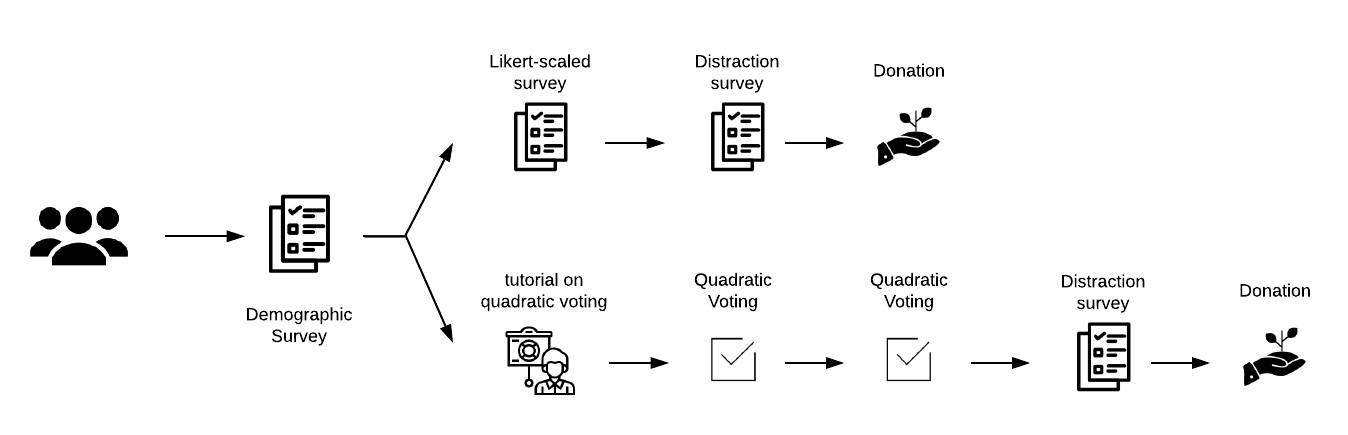
\includegraphics[width=\textwidth, keepaspectratio=true]{content/image/exp1_flow.png}
    \caption{
        Experiment one conducted between subjects. Participants were divieded into two groups. Participants that took the upper path is the Likert Group and the alternative is the QV group.
    }
    \Description[Image describing the flow for experiment 1]{Image describing the flow for experiment 1}
    \label{fig:exp1_image_flow}
\end{figure}

At a high level, 
we summarize the experiment flow 
in Graph \ref{fig:exp1_image_flow}.
The experiment consisted four steps:
To begin the experiment, 
participants filled out the demographic survey.
Based on the demographics,
participants completed one form of opinion collection,
highlighed as the yellow box
in Graph \ref{fig:exp1_image_flow}.
After that, 
participants filled out another survey,
the distraction survey,
to divert their attention before they complete the final task.
The final task asked participants to do a donation.
Now we explain each section in detail.

Prior to starting the experiment,
participants were told that 
this study aims to understand their opinions 
toward societal causes and will be asked to complete a donation task.
During the demographic survey, 
we collected the participant's gender, ethnicity, age range, household income level, 
education level, and current occupation.
Based on the age and education level,
we divided participants into seven groups
and made sure each group contained the same distribution
as the US 2019 census.
These seven groups can be further categorized as
the Likert Group (Group 1) and the QV Group (Group 2 to 7).
The Likert Group, shown as the upper path in the shaded aread of Graph \ref{fig:exp1_image_flow}, 
revealed their opinion using a Likert scale survey.
The QV Group, shown as the lower path in the shaded aread of Graph \ref{fig:exp1_image_flow}, 
revealed their opinions by completing two QVs, each with a different numbers of voice credit.
The reason why we divided the QV Group into six subgroups
is to answer research question three, 
that is whether the number of voice credits impacts the outcome.
These two voice credits that participants experience 
are drawn from three possible values: $N \times O$, $N^1.5 \times O$, $N^2 \times O$, 
where $N$ is the number of options in the survey, 
and $O$ is the number of levels, 
excluding neutral on the Likert scale survey. %not sure if this is clear
In our case, with nine options ($N=9$) and
used a five-point Likert scale survey ($O=4$), 
thus three values would be $36$, $108$, and $324$.
With these three possible values, 
we choose two for each of the six subgroups.

In the Likert group, 
the survey looks identical to a typical five-point Likert scaled survey.
We assume participants have prior knowledge in Likert surveys.
Participants were presented with the nine societal causes, 
and were asked the importance each of these causes: 
With options ranging from ``Very important'' to ``Very Unimportant.''

In the QV group, 
participants were asked to watch 
a prerecorded tutorial video of QV's concept 
and how to operate the QV interface.
Participants are granted unlimited time 
to interact with a demo QV interface. 
This process is demonstrated as 
``tutorial on quadratic voting'' 
in Graph \ref{fig:exp1_image_flow}.
To ensure that participants paid attention to the video and understood QV, 
they were asked to answer at least three of the five multiple-choice questions 
correctly to continue with the survey.
Once participants passed the quiz, 
paticipants will be given voice credits of either 36, 108 or 324.
They will vote in QV using these voice credits 
with the nine options identical to those in the Likert Group.
Participants would repeat this action using a different set of voice credits.
These two QVs are shown as two QV icons in Graph \ref{fig:exp1_image_flow}.



After both groups of participants completed their surveys in the opinion collection stage, 
they finish a short answer question
that allowed them to express their thoughts 
related to another set of societal issues.
These societal issues are unrelated in the previous stage,
and are designed to distraction participants.
We do not want participants to connect their survey responses
to interfere with their behaviors during the donation task.

Finally, 
we ask participants to perform a donation in the final stage.
This task persented nine organizations,
each referring to one of the nine societal causes
that we listed during the opinion collection phase.
Partcipants can donate up to 35 dollar 
to any of these organizations.
To ensure incentive compatibility, 
participants do not donate imaginatively.
Participants are aware that every one in 70 participants would win 35 US dollars.
Assuming winning the 35 US dollars, 
the participants were asked 
if they would want to donate some money 
to any of the nine charity groups.
Participants are also aware that 
they keep the remaining amount of undonated money 
if they win the lottery.
Further, participants are aware that 
the research team will match one dollar to each one dollar 
they donated to an organization.
This setup means the donation carried an underlying cost.

To minimize the difference across groups in the study, 
we use the same prompt across Likert scaled survey, QV, and the donation task.
We explicitly tell the participants that 
there are limited resources in the society, 
and people have different preferences 
in how resources should be allocated and ask the participants, 
``What societal issues need more support?''

To ensure that the nine societal causes 
covered a broad spectrum of categories.
We used the categorization of charity groups on Amazon Smile, 
a popular donation website that has accumulated over 100 million dollars of donations, 
as our topics of the societal causes.
The categories include (1) Pets and Animals, (2) Arts, Culture, Humanities, (3) Education, (4) Environment, 
(5) Health, (6) Human Services, (7) International, (8) Faith and Spiritual, and (9) Veteran. 
Within each of these categories, 
we select one charity organization from Amazon Smile 
as the representation of the subject matter used in the donation task.

\subsection{System Design}
We using Python Flask for the back-end, Angular for front-end, 
and MongoDB for database storage to construct the voting system. 
The experiment source code is publicly available \footnote{Not yet public}, 
and so is the QV interface as a stand-alone repository \footnote{https://github.com/hank0982/QV-app}.

\begin{figure}[htpb]
    \centering
    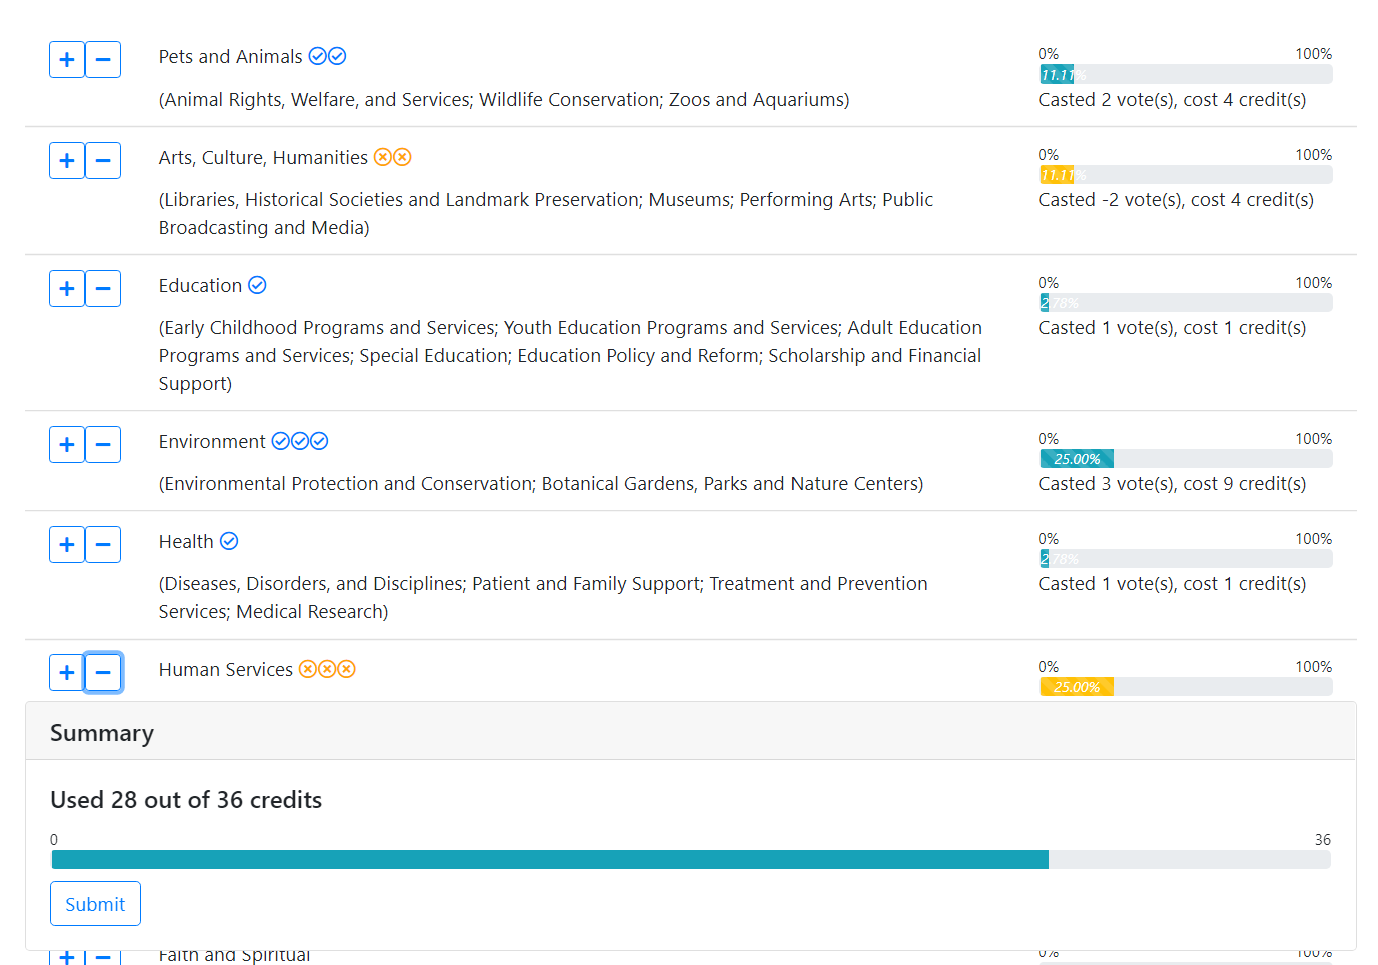
\includegraphics[width=0.7\textwidth, keepaspectratio=true]{content/image/qv-donation.png}
    \caption{
        The QV voting interface used across both experiments. 
        We omit the prompt in this figure.
        After mutiple iterations (details in the Appendeix), 
        the interface allows participants to vote, 
        with real time feedback of how the votes allocats. 
        The progress bar implementation 
        were inspired by knapsack voting interface by \textcite{goel2015knapsack}.
    }
    \label{fig:qv_donation}
\end{figure}

The QV interface, is shown in Figure \ref{fig:qv_donation}.
The body section is the voting panel
that contained all options to vote for.
To the left of each option, 
participants vote using the plus and minus buttons.
Buttons are disabled 
if the number of voice credits 
does not permit the next vote.
A bar on the right of the option 
shows the proportion of voice credits 
used to that option with text associated with the visual.
The different colors and the icons 
to the right of each option 
exhibits the number of for or against 
that currently devoted to an option.
The summary panel always 
floats at the bottom of the page 
to ensure visibility.
A progress bar shows the number of voice credits 
that the participants have and had not used.\par
\subsection{Experiment 1 Results} \label{results-1}
\subsubsection{Quantitative Analysis Results}

% -- raw data
%     describe the dataset, total # of participants in each group before and after dataset cleaning, demographics of each group;
    
%     donation descriptive statistics: perc of non-zero donation, total donation amount comparison across groups (discuss our test of checking if other factors impact total donation amount -> absolute vs. normalized donation amount), donation distribution across topics between groups
    
%     QV & Likert votes descriptive statistics: votes distribution per topic across groups, budget usage distribution across QV groups
    
% -- data transformation to alignment measurement
%     describe the calculation of cosine similarity angle theta
%     show histogram and other descriptive statistics of the angel data
    
% -- Bayesian formulation
%     why Bayesian
%     the type of analysis question
%     choice of the likelihood function
%     choice of prior distributions
    
% -- Results analysis
%     Tools: PyMC3, MCMC, NUTS
%     Describe fitted values & convergence (trace plots)
%     Describe effect size analysis for comparing Likert and QV
%     Describe effect size analysis for comparing across QVs
    
\subsubsection{Qualitative Analysis Results}
We ask participants to provide a freeform text response on the reason why they made the choices they made
when participants filled out the Likert scale survey or QV survey,
Of all surveys ($N=394$) across both groups, most participants filled out the surveys ($N=331$) based on what they think are the most important issues to them. %84 percent
Besides, a small portion of participants ($N=30$) used their instincts when replying to the survey.
Some participants either think that every aspect is important ($N=7$) or that resources should be equally distributed ($N=7$).

For the participants that said they reply based on what they think is most important to them, 
participants usually perform an ``electing'' over a handful of issues first and then indicate their preference.
% limitation at showing intensity @ Likert
However, we see a few instances in the Likert group where participants would claim one to two options as the most critical causes but electing three or more ``very important''.
For example, P09a47 mentioned, ``I think the environment education and healthcare should be our top priorities right now. Other issues are also important but not as much so.''
while filling out Education, Environment, Health, and Human Services as ``Very important.'' 
Pd80fc mentioned, ``[I] think health and the environment are important'' while putting Pets and Animals, Arts, Culture, Humanities, Environment, and Veteran. as ``Very important.'' 
Though it is unclear why there is this discrepancy, one participant (P9b3ae
) explicitly mentioned ``[\textellipsis] I would answer otherwise, if there were other options, such as not much, or a little bit.''
Similar issues were not present in the QV Group responses.
Participants were able to express more fine-grain preferences.
P1fee1 mentioned, ``I think health and human service are important and beneficial for society.'' while voting six votes for health and five votes for human services. This indicates that despite being ``important'', there is still a difference in weight and shadowed the limitation of Likert scaled survey, where people can be limited by the options they were given.\par

Despite only occurring once (P1d659), we think the term ``voting'' might motivate participants to consider how a collective decision was made.
This participant mentioned ``[\textellipsis] I thought a lot of people would probably support faith and spiritual ecatagory  so I watned to try to counterbalance that by voting against it.'' The participants are willing to pay the cost by devoting fewer votes for issues they care and vote against specific ballots. This behavior is not possible in a Likert scaled survey.\par

To understand how participants in QV voted, we also analyze how participant's responses changed when the number of voice credits changed. 
If the number of voice credits increased, as expected, some participants uniformly increased the number of votes across all nine options, stating that they try to be fair. Also, logically, other participants would devote the additional voice credits to the items of their likes or dislikes. 
It is, however, fascinating to identify how additional credits pushed participants to express more fine-grain preferences.
For example, some participants that had a drastic increase of voice credits, from 36 to 324 voice credits, expressed devoting some options that originally had zero votes. 
P2d9da stated, ``Because now that I have a lot more credits, I felt that I could vote on more issues that mean something to me.'' The participant initially only voted for Environment; however, with 324 votes, the participants voted for all but Faith and Spiritual. This supports our quantitative finding that a limited amount of voice credits suppressed the performance of QV. Participants also reported being freer and submitted more fine-grain opinions. As one participant (P54f23) responded: ``The greater voice quantity allowed me to vary the differences in choices'' more and similarly Pcc4aa reported, ``with more credits i can show what i really like.''

On the contrary, participants are forced to downsize their preferences if credits decreased. Many participants voiced their need to make tradeoffs. P9e5e6 said, ``I think I covered the bare basics.'' and Pe37f2 said, ``Less to go around, so had to knuckle down and allocate the most to what I think is most important.'' Again, this means that it is crucial to have enough points if we want to reflect participant's preferences and they're intensity accurately.

One thing to notice is participants scaled their preferences based on the number of total voice credits. Even though voice credits are one single unit and do not carry any weight, when total voice credits increase, the value of each voice credit devalued, vice versa. P24194 stated, ``I had fewer credits so each vote seemed more expensive.''

This set of qualitative analysis support the quantitative finding that the number of voice credits impacts the performance of QV and there is a need to find the best way at deciding \textit{what} the number of voice credits should be.
\section{Methods -- experiment Two: Importance of Video Elements}
\label{method-2}
The first experiment answered RQ1 and showed that QV aligned closer to the participants' true preferences compared to Likert scale when choosing among $K$ independent options of the same subject matter. To strengthen our results and examine the generalizability of QV, we designed a second experiment to answer our second research question: \begin{quote}RQ2: How do QV responses align with people's true preferences compared to Likert scale responses in a survey where survey respondents choose among $K$ dependent options that jointly contribute to the same topic?\end{quote} To give an analogy: the first experiment is related to preferences among ice cream, cakes, and puddings as desserts, whereas the second experiment assesses what an individual cares more about when choosing ice cream -- the flavor, texture, or ingredients. Since relationships and interactions among ballot options may impact how users make trade-offs, we want to examine if the results from QV also align better with people's true preferences than Likert scale in the use case of RQ2.

We hypothesized that QV would outperform Likert in accurately eliciting participants' true preferences in the new setting. We changed the application domain from public policy to HCI since HCI user studies often rely on eliciting preferences from users to inform designs that involve trade-offs and in turn create better user experiences. These characteristics made HCI studies an excellent domain to test out QV. To verify our hypothesis, we designed a within-subjects study that elicited participants' preferences on different video elements using QV, Likert, and a pricing task. 

% Second, we changed the \textit{relationships and interactions} among items in the survey. In experiment 1, the different societal causes (items) impacted the society (topic) on their own without influencing each other. But experiment two focused on ballot items that represented different \textit{aspects} that jointly contributed to the same subject matter and may interact with one another, a typical case in the HCI domain. 
% We hypothesize that the latter case is more challenging for the participants to express accurately. Thus, if QV could outperform Likert in such cases, it will broaden the use cases for QV.

% Lastly, the second experiment focused on a setting that surveyed matters with a more tangible and immediate outcome to the participants, a common scenario in HCI studies, as opposed to matters with a more abstract and further-in-the-future impact. This difference may also impact the relative performance of QV and Likert. 
% Our last change made the second experiment a within-subject study to understand how the same individual's expression differs using different survey tools.

In this section, we first explain how we selected video streaming experience as the HCI study scenario. Then, we demonstrate the experiment workflow accompanied by the interfaces of the experiment. Finally, we explained the analysis approach.

%<---------------------------->%
% HCI Experiment background
%% Video HCI experiments
%% Selection of the five elements and their definitions
%% The goal of this HCI experiment is to find elements that impact participants most.
%<---------------------------->%
 
\subsection{Choice of HCI study} \label{exp2-hci}
We set out to find a typical HCI study where UX/UI researchers survey users to understand what features to prioritize. In the end, we decided to use the research scenario of understanding users' preferences among various video and audio elements under network or monetary constraints \cite{molnar2013comedy, oeldorf2012bad}.
% On the one hand, we wanted to avoid creating an entirely new HCI study that required sophisticated verification. On the other hand, reproducing a prior HCI study that used Likert surveys can be costly and difficult because of the limited access to the devices, designs, or interfaces used in the study. Therefore, we developed new research based on prior research but with a new research question and study design to maintain ecological validity.

Research on video and audio elements of video playback from the lens of HCI is relatively mature. Understanding how users with bandwidth constraints made trade-offs across multiple videos and audio elements \cite{molnar2013comedy, oeldorf2012bad} is a typical example for which of the $K$ dependent options of the same topic would people prioritize under constraints. \textcite{oeldorf2012bad}, for example, conducted a study to examine the differences in participants' perceptions between three video bit rates, three video frame rates, and two audio sampling rates across three types of video content via a 5-point Likert scale. 
% Participants rated the overall quality, video quality, audio quality, and enjoyment level  in each condition. The study derived the conclusions from analyzing the means and standard deviations of the Likert survey results. This HCI experiment is a typical study to explore which one or some of the $K$ elements to prioritize under constraints.
% Researchers provided insights to topics including multi-media conferencing \cite{watson1996evaluating}, video-audio perception \cite{chen2006cognitive, molnar2015assessing}, and, more specifically, trade-offs among various video and audio elements under network or monetary constraints \cite{molnar2013comedy, oeldorf2012bad}. understand how users with bandwidth constraints made trade-offs covering a broad set of elements across multiple videos and audio elements. They 

We proposed a similar user research topic as in \textcite{oeldorf2012bad}'s study. We designed the experiment to answer the following question: ``Given a video with unsatisfying quality, under limited bandwidth, how should the bandwidth be allocated to enhance the five visual and audio elements, including motion smoothness \cite{huynh2008temporal}, audio stability \cite{hardman1998successful}, audio quality \cite{knoche2008low}, video resolution \cite{knoche2005can}, and audio-video synchronization \cite{steinmetz1996human}, to obtain an acceptable video streaming experience from the viewers' perspective?'' We selected the five video elements based on prior work. For their detailed definitions, please refer to \Cref{elem_def}. To our knowledge, no prior work has studies the combination of five elements in a single experiment.

Prior work suggested that the type of video affected users' perceptions for video elements. In this experiment, we used a 90-second weather forecast video for the United States. We chose a weather forecast video for two reasons. First, the concept of a weather forecast is generic and universal. The terms used in the weather forecast are usually easy to understand. Second, since we are studying both audio and visual elements, we wanted a video that conveyed information via both visuals and speech. In a weather forecast video, the meteorologist usually spoke aloud the weather while pointing at visual cues such as icons and numbers.
% There is no prior literature that looked at five combinations in a single experiment and studied them together, to the best of our knowledge. Hence, this is a valid HCI-related research question. We are also aware that these video elements' importance relies heavily on the type of video being served. 
% Video clips such as sports can contain specific jargon, while movie clips can be unfamiliar to some and not to others. a large amount of visualization but also provided information through speech. Drama and talk shows, for example, would lean towards visual elements or audio elements. Finally, visual and audio elements in a weather forecast complement each other. 

In the next section, we describe how we conducted the video elements trade-off experiment to compare QV and Likert scale's ability in truthfully reflecting users' preferences across the video elements.
% answering the research question in identifying the video/audio elements that impact participants' streaming experience the most.



\subsection{Experimental Flow}
We recruited participants on Mechanical Turk through the CloudResearch platform \cite{litman2017turkprime}. Like our first experiment, we used a pre-survey to match the participants' distribution with the U.S. population in age and education based on 2018 US census estimates. The average completion time was 35 minutes 42 seconds and all participants received \$6 as base pay and a bonus up to \$2. All participants followed six steps. The six steps were (1) demographic survey, (2) tutorials and attention checks, (3) a video playground, (4) Likert and QV surveys, \tc{(5) a filler task}, and (6) a design task. Now we explain the six steps in detail. \tc{We provide the experiment flow diagram in the appendix and present the experiment protocol as supplementary materials.}

\textbf{Step 1. Demographic Survey} We greeted participants with a consent form. In the consent form, we presented the goal of the study as understanding how people think about the importance of the different elements during video streaming. We did not reveal to the participants that this experiment aimed to compare Likert and QV until they completed the survey. Once participants gave their consent, they would fill out a demographic survey that contained questions identical to those in the first experiment.

\textbf{Step 2. Tutorials and Attention Checks} In step two, we provided two tutorials to the participants. All participants would first read through a tutorial that defined the five video elements used in the experiment, via textual explanation and pairs of video examples. On the next page, they needed to answer five multiple-choice questions about the definitions of video elements and two attention checks designed to see if audio and video played fine on the participant's device. Participants qualified for continuing the experiment only if they answered fewer than two questions incorrectly. This step made sure participants fully understood the terminologies used in the rest of the experiment.
% In this tutorial, for each video element, we showed a pair of videos side-by-side for participants to compare how the same video would differ if a particular element were perfect and when the element is of lousy quality. 

Participants then moved on to a tutorial on how QV works, with a short instructional video supplemented with text. They had a chance to play with a QV interface similar to that in \Cref{fig:qv_donation}. Once the participants were confident that they understood QV, they needed to complete the same QV quiz in experiment one. The system disqualified a participant immediately if they answered two or more questions wrong.

\begin{figure}[htpb]
    \centering
    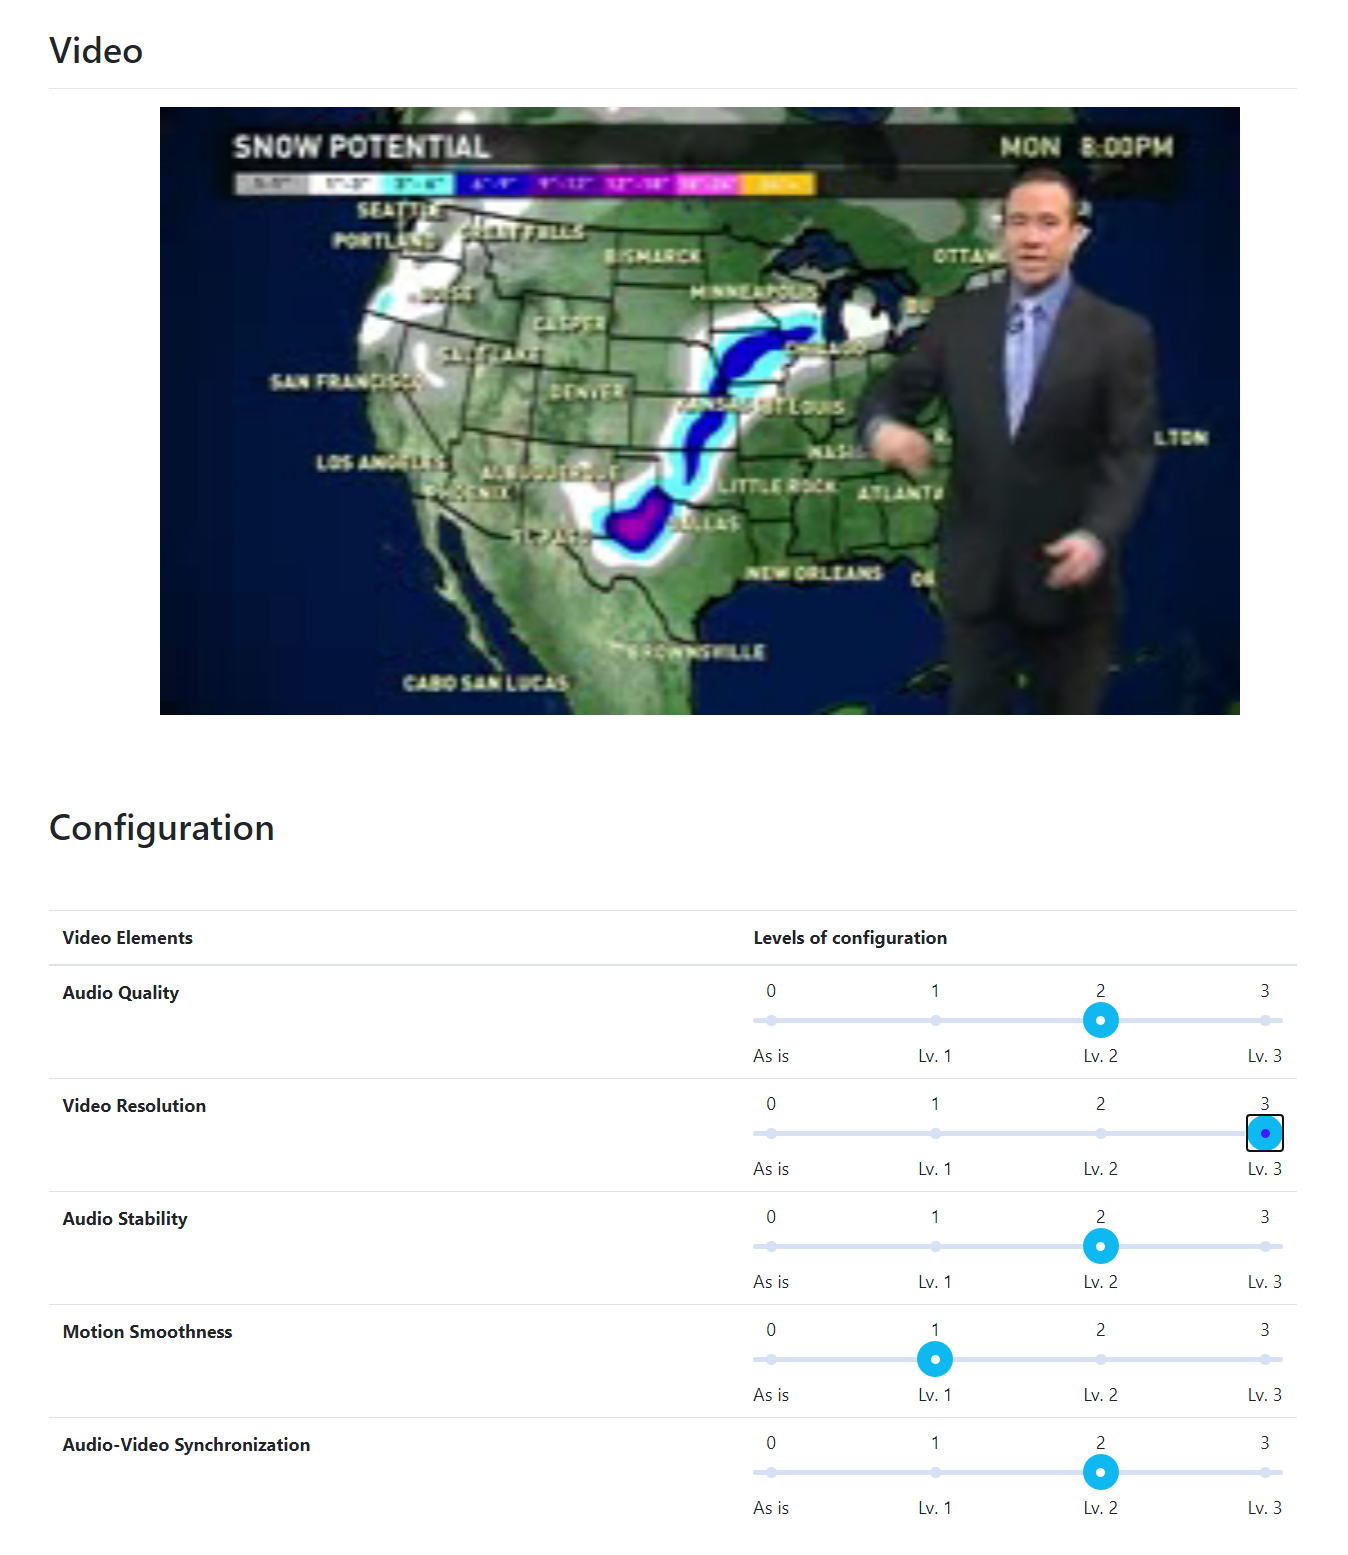
\includegraphics[width=0.8\textwidth, keepaspectratio=true]{content/image/video_playground.png}
    \caption{
        The real-time video element interface allows participants to adjust video playback elements and understand how differences in the elements impact their viewing experience. We selected four levels of quality settings for each element according to prior research, ranging from an unacceptable quality to a good quality. The technical details of this implementation are described in ~\cref{appx_video_interface}.
    }
    \label{fig:exp2_playground}
\end{figure}


\textbf{Step 3. Video Playground} To increase this experiment's fidelity, we framed the study as a market research initiative by a fictional company (participants were not aware that the company was fictional), with a goal to provide a video-streaming product in cars using satellite-based Internet. We first showed the participants the ``current prototype" of the company's streaming service, which simulated what a weather forecast video played under limited bandwidth would look like, with all five elements at the worst quality in the range we designed to study\footnote{Motion smoothness: 2.5 fps; Audio stability: 20\% packet loss rate; Video resolution: 120x90 at 32 kbit/s; Audio quality: 8kHz sampling rate; Audio-video synchronization: visuals play 2000ms ahead of the audio}. 
% After experiencing the current prototype, the participants moved on to the next page.

To help participants better understand the impact of various enhancement levels for each element on the current prototype, we led them to a video playground shown in \Cref{fig:exp2_playground}. This playground allowed participants to use the control panel to adjust the levels of enhancements for all five video elements and see real-time changes in the video on the top of the page, i.e., the video played in the most recent combination of quality levels. Participants could pause and play the video at any time, and replay the video as many times as they choose. We encouraged participants to test out different combinations freely in this playground to help them understand the impact of each element and how the five elements interact. We asked participants to describe how changing the elements impacted their experience in a free-form text question to make sure participants did experience different settings.
% It is important to note that this interface is important because we asked participants to elicit preferences among the different \textit{perspectives} of the same subject matter. Each of these perspectives might not be independent of one another.
% We then instructed them to explore how various enhancement levels on different elements in the current prototype would improve their viewing experience. 

% This interface showcased a weather forecast video on the top of the page. 
% Participants can toggle any of these five elements to any of the four levels at any time. According to the quality levels the participants set, the video playback will immediately apply those changes. We .

For each element, we provided a slider with four levels, Level 0 at the lowest quality and Level 4 at the highest. We designed the intermediate levels based on prior research such that the changes between each level of an element had a quasi-linear impact on viewers' perception. The four levels of the five video elements are listed below, from Level 0 to Level 3:
\begin{itemize}
    \item Motion Smoothness \cite{huynh2008temporal}: 2.5 fps, 6.25 fps, 8 fps, and 25 fps
    \item Audio Stability \cite{hardman1998successful}: 20\%, 10\%, 5\%, and 0\% probability in packet loss
    \item Video Resolution \cite{knoche2005can}: 120x90 at 32 kbit/s, 168x126 at 64 kbit/s, 240x180 at 96 kbit/s, and 240x180 at 224 kbit/s; encoded in the WMV2 (Windows Media Video 8) codec 
    \item Audio Quality \cite{knoche2008low, noll1993wideband}: 8kHz, 16kHz, 24kHz, 32kHz; encoded using the AAC (Advanced Audio Coding) codec
    \item Audio-Video Synchronization \cite{steinmetz1996human}: 2000ms, 1250ms, 750ms, 0ms; visual ahead of audio
\end{itemize}


\textbf{Step 4. Surveying Preferences} After experiencing how different enhancements on the five video elements impacted their viewing experience, we collected participants' opinions on how critical the improvements on each video element in the current prototype were for them to understand the weather forecast video. Participants completed  a QV survey and a Likert scale survey in a randomized order to prevent ordering effect. Since this was a within-subjects study, we randomized the display order of the elements on the surveys to minimize carryover effect and ordering effect. The QV interface was similar to that in experiment one. We designed the credit budget to be 100 voice credits, the best option based on experiment one, i.e., $K^2 x O$, where $K=5$ and $O=4$ in this case.

\tc{
\textbf{Step 5. Filler Task} Before moving on to the task for eliciting the participant's true preferences, we designed a survey as the filler task that asked about participants' consumption preferences across different subscription tiers for several well-known streaming services. This survey aimed to prevent participants from translating their survey responses directly to the next task. We told participants that this survey results would be an important part of the next task.}

\textbf{Step 6. Design a Product} To capture a participant's true preferences on how much they \textit{value} each of the five video elements, we created an incentive-compatible product design task to elicit their true willingness-to-pay for the elements. To create a high fidelity scenario, we told participants that the system assigned them into the designer group, and their job was to design a streaming service for cars via satellite internet. They should design and price their product such that another participant from the buyer group (fictional but the participants were not aware), who we claimed to have matched for them based on demographic information and the consumption preference survey, would be willing to purchase the product. We emphasized that their product should be affordable and should allow the buyer to understand the weather forecast video. To incentivize the participants, we offered them 10\% of the final price they proposed as their bonus if the buyer decided to purchase their product.

% The instruction also told participants to consider that each element is associated with a cost, and the buyer will need to pay each element's cost. We told participants that if the buyer decides to purchase the product, they will receive 10\% of the final price they proposed as their commission. 

We guided participants to complete the task in two steps.  In the first step, participants needed to select one of the two qualities for each video element, a lower quality and a higher quality, and ``assemble'' the product. Quality one refers to level 0 in the playground, the worst one they had experienced. For quality two, we selected the quality levels in the playground that matched what prior research showed to be the ``acceptable level''\footnote{Motion smoothness: 6.25 fps; Audio stability: 10\% packet loss rate; Video resolution: 240x180 at 96 kbit/s; Audio quality: 16kHz sampling rate; Audio-video synchronization: visuals play 750ms ahead of the audio}. Participants saw real-time changes to the video as they updated the qualities. Participants were essentially making a binary decision of whether a video element was ``important'' or ``not important'' for them, and equivalently for the buyer that had similar preferences as them. 
% This binary design prevents us from bounding participants' choices when provided a slider. 

In the second step, participants set a price they thought to be reasonable for each of the five elements between \$0 - \$4 based on the qualities they selected and how much they thought the buyer would value them. The sum of these prices was the total price of the product. We reminded participants throughout the task that the higher they priced the elements, the more their bonus could be. However, if they overpriced any element from the buyer's perspective, the buyer might not purchase their design and they would fail to gain any bonus. 

The goal of this design was to elicit the truthful willingness-to-pay for each participant as the their true preferences. Our set-up was incentive-compatible and the best strategy for the participants was to price based on how they themselves valued each of the elements. If they priced the product higher than their accurate valuations, the ``buyer'' with similar demographic and consumption preferences as them would reject their proposal, given that the buyer would likely value the elements the same way. Vice versa, if the participants set their prices to be lower than their actual willingness-to-pay, they would lose out on earning a higher bonus.

% Notice that instead of giving participants the power to select the quality over various levels as they did in the video playground in step three. We only provide two qualities for each video element. 

\subsection{System Design}
We reused the QV interface from experiment one in our second experiment. To create real-time adjustments in video qualities, we pre-generated video-only and audio-only files of different qualities. When a participant changed an audio or video quality setting, the system served the correct combination of video and audio files. We used JavaScript to adjust the video-audio synchronization in the front-end at real-time.

This design balanced the need for a high network speed to stream every configuration from the server and the need for a powerful client to compute the video and audio qualities. The experiment source code for experiment two is publicly available \footnote{https://github.com/dummy\_url}. More details of the system implementation are provided in \Cref{appx_video_interface}.

\subsection{Analysis Method}

Since RQ2 is also about the degree of alignment, similar to RQ1, we followed a similar analysis approach as described in \Cref{method_exp1}. In experiment two, we compared the alignment between survey responses with the prices set in an incentive-compatible scenario. We used the same definition of ``alignment" and the same metric for alignment, cosine similarity angle, as explained in \Cref{alignment_metric}. For the Likert group, we mapped the ordinal responses into a vector where the result for each video element ranges from $-2$ to $2$. For QV, the vector contains the number of votes for each video element. Then, we computed the cosine similarity angle between a Likert or QV vector and the absolute prices set by the same participant,.

Once we obtained the two sets of cosine similarity angles, one for Likert and one for QV, we applied the same Bayesian formulation detailed in \cref{exp1:The Bayesian Model} to model the mean cosine similarity angle in both groups. Then, we compared the two distributions to see if they how far they are apart.
\section{experiment Two Results} \label{results-2}
In this section, we first describe the participants' demographic in the second experiment. Then, we present descriptive statistics for the raw data. Lastly, we discuss results from our Bayesian analysis.

\subsection{Participant Demographics}
We collected 101 complete responses in the second experiment. We removed 8 poor-quality responses where participants responded to the qualitative questions facetiously and put the same survey rating across all video elements. Among the remaining 93 participants, 55 of them identified as male and 38 as female. Around 80\% of the participants were White, 13\% were Black or African American, 5\% were Asian, and the remaining 2\% preferred not to disclose their racial information. Similar to experiment one, we aligned the participants' age and education level distribution to match that in the US 2018 census estimates~\cite{census2018}, as shown in \Cref{table:demo_exp2}.

\begin{table}
  \centering
  \caption{experiment two sample demographics statistics align closely with 2018 US census. } \label{table:demo_exp2}
  \sisetup{
    table-number-alignment = center, 
    table-figures-integer = 2, 
    table-figures-decimal = 2,
    round-mode = figures,
    round-precision = 3,
    detect-weight=true
  } \begin{tabularx}{0.5\textwidth}
    {@{}>{\raggedleft\arraybackslash}X>{\bfseries}SS@{}}
    \toprule
    Demographics & {Sample (\si{\percent})} & {Census (\si{\percent})} \\
    \midrule
    \textsc{\bfseries Education} & &\\
    No High School & 4.30 & 10.22  \\
    High School & 27.96 & 27.73  \\
    College  Associate & 31.18 & 33.09  \\
    Bachelor's Degree and above & 36.56 & 33.09  \\ 
    \textsc{\bfseries Age} & &\\
    18--24 & 9.68 & 13.65  \\
    25--39 & 39.78 & 30.74  \\
    40--54 & 27.96 & 28.32  \\
    55--69 & 22.58 & 27.29  \\
    \bottomrule\end{tabularx}
\end{table}

\subsection{Descriptive Statistics}

As shown in \Cref{fig:likert_exp2} and \Cref{fig:qv3_exp2}, on an aggregated level, participants expressed similar relative preferences across the five video elements in both Likert and QV. Audio quality ranked the highest in both cases, while motion smoothness and audio-video synchronization had the lowest ranks. While the aggregated preference were similar between Likert and QV, we will discuss their differences on an individual participant level in the next subsection. Similar to experiment one, a majority of the Likert response distributions skewed to the left; in contrast, QV response distributions approximated a Normal distribution. With a budget of 100 voice credits in QV, 57\% of the participants used at least 98\% of the budget and 82.8\% of them used over 90\% of the budget, suggesting that most participants actively made use of the majority of the budget.

\begin{figure}[htpb]
\centering
\begin{minipage}[b]{0.44\linewidth}
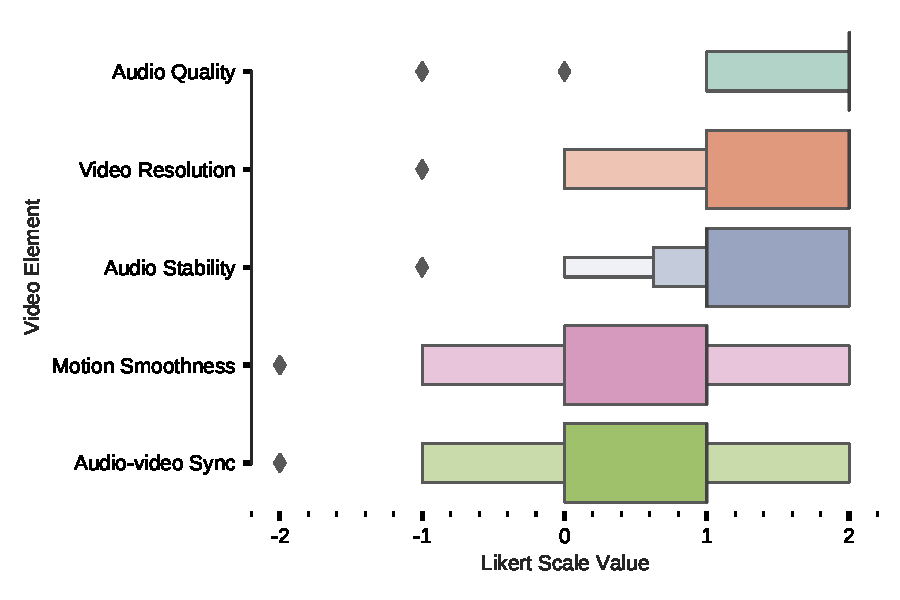
\includegraphics[width=\textwidth, keepaspectratio=true]{content/image/likert_distribution_per_element (1).pdf}
    \caption{
      Distribution of Likert scale survey responses per video elements in Boxen plot. 
      Each level from -2 to 2 corresponds to 
      ``Very unimportant'', ``Unimportant'', ``Neutral'', ``Important'', and ``Very important''.
      The distributions of different elements vary in their shapes, suggesting that participants showed their relative preferences even in the Likert group.
    }
    \Description[Distribution of Likert Responses per element for experiment two in Boxen plot]{Distribution of Likert Responses per element for experiment two in Boxen plot}
    \label{fig:likert_exp2}
\end{minipage}
\quad
\begin{minipage}[b]{0.52\linewidth}
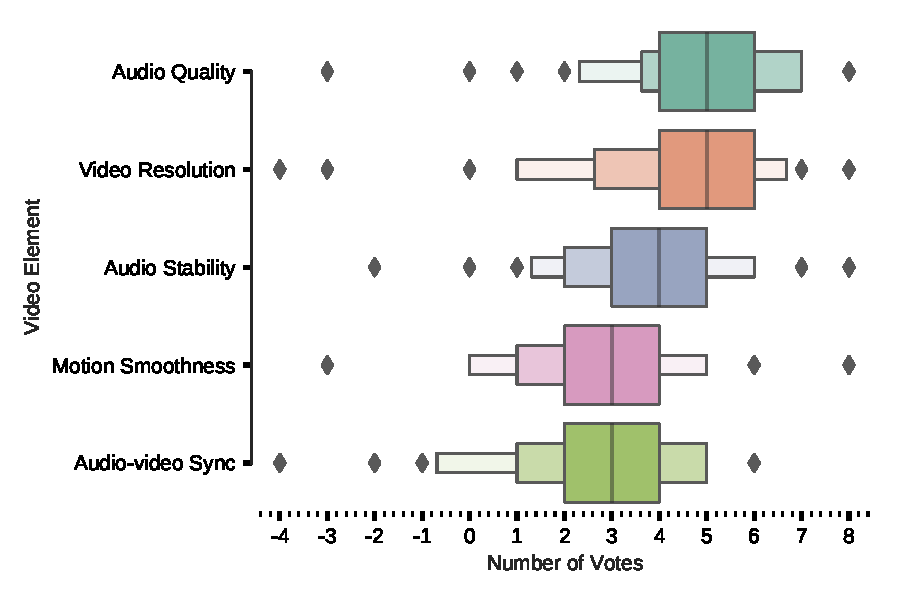
\includegraphics[width=0.9\textwidth, keepaspectratio=true]{content/image/qv_distribution_per_element.pdf}
    \caption{
      Distribution of QV responses per video element in QV in Boxen plots. The maximum possible number of votes on an element was 10 votes given 100 voice credits. Most distributions in all three QV set-ups follow a normal distribution. 
    }
    \Description[Distribution of QV Responses per element for experiment two]{Distribution of QV Responses per element for experiment two}
    \label{fig:qv3_exp2}
\end{minipage}
\end{figure}

\begin{figure}[ht]
    \centering
    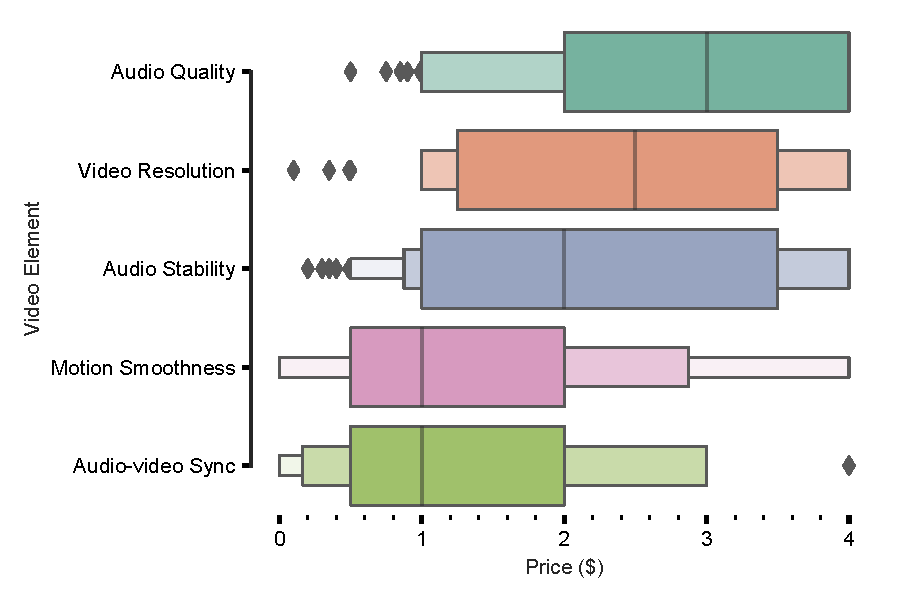
\includegraphics[width=0.5\textwidth, keepaspectratio=true]{content/image/price_distribution_per_element.pdf}
    \caption{
      Distribution of prices set by participants per video elements in Boxen plot. 
      Prices ranged from \$0 to \$4. Compared to the survey response distributions, elements with a higher rating of importance in surveys also had higher prices during product design.
    }
    \Description[Distribution of prices per element during the product design task in experiment two in Boxen plot]{Distribution of prices set for each element in experiment two in Boxen plot}
    \label{fig:price_exp2}
\end{figure}


Set prices for the five video elements exhibited similar patterns as the survey responses on an aggregated level (\Cref{fig:price_exp2}). Compared to the survey response distributions, elements with a higher average rating of importance in surveys also had higher average prices during product design. Since we instructed participants during price-setting that the buyer would be willing to pay more for the element that they value more, the alignment of preferences on an aggregated level between surveys and prices indicated that the participants kept our instruction in mind when they decided on the prices.


Similar to experiment one, we are interested in the degree of alignment between survey responses and prices set in an incentive-compatible scenario on an individual level. \Cref{fig:topic_covariate_exp2} visualizes the estimated correlation between normalized Likert or QV responses and normalized prices. All elements had a trend line with a positive slope, suggesting potential positive correlations. QV responses seemed to {\change{have}} a more positive slope with prices compared to Likert responses, indicating a possibly better alignment. Next, we present statistical support for this phenomenon.

\begin{figure}[htpb]
    \centering
    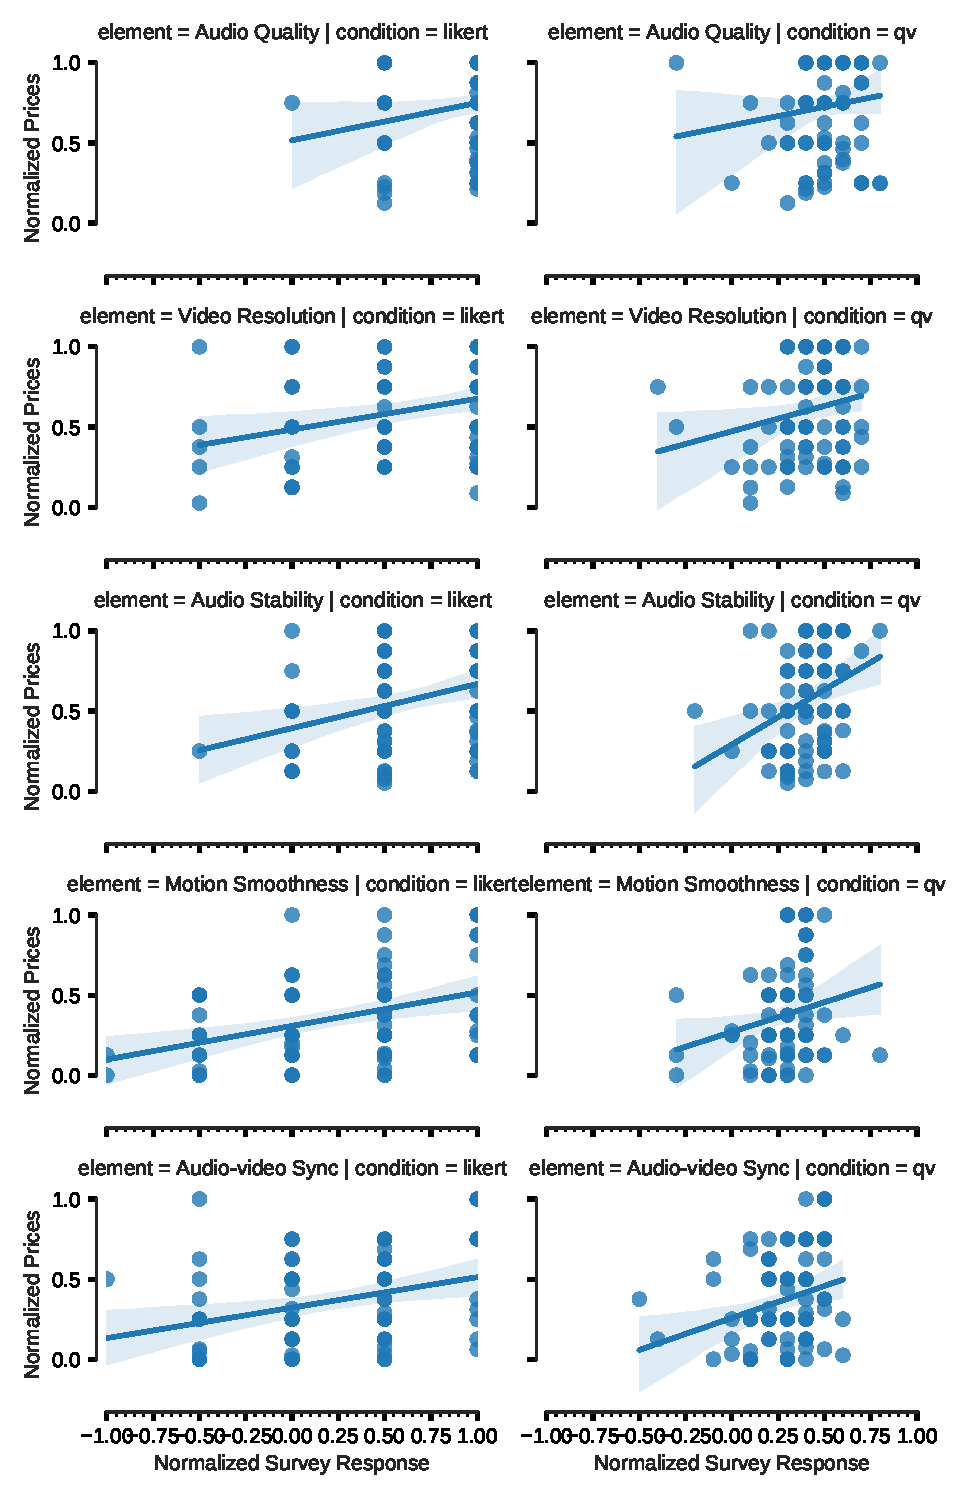
\includegraphics[width=0.6\textwidth, keepaspectratio=true]{content/image/correlation_per_element.pdf}
    \caption{
      Scatterplots showing the correlation between participants' normalized survey response and normalized prices for five video elements in the Likert survey and QV survey. Each row is one topic, and each column is one survey condition. \textbf{The main finding} is: all elements had a trend line with a positive slope, indicating potential positive correlations. QV responses seemed to {\change{have}} a more positive slope with prices compared to Likert responses, indicating a possibly better alignment.
    }
    \Description[Correlation scatterplots between normalized survey responses and normalized prices for experiment two]{
      Scatterplots showing the relationship between participants' normalized survey response and normalized prices for each of the five video elements in Likert and QV.
    }
    \label{fig:topic_covariate_exp2}
\end{figure}


\subsection{Bayesian Analysis Results}


\begin{figure}[htpb]
  \centering
  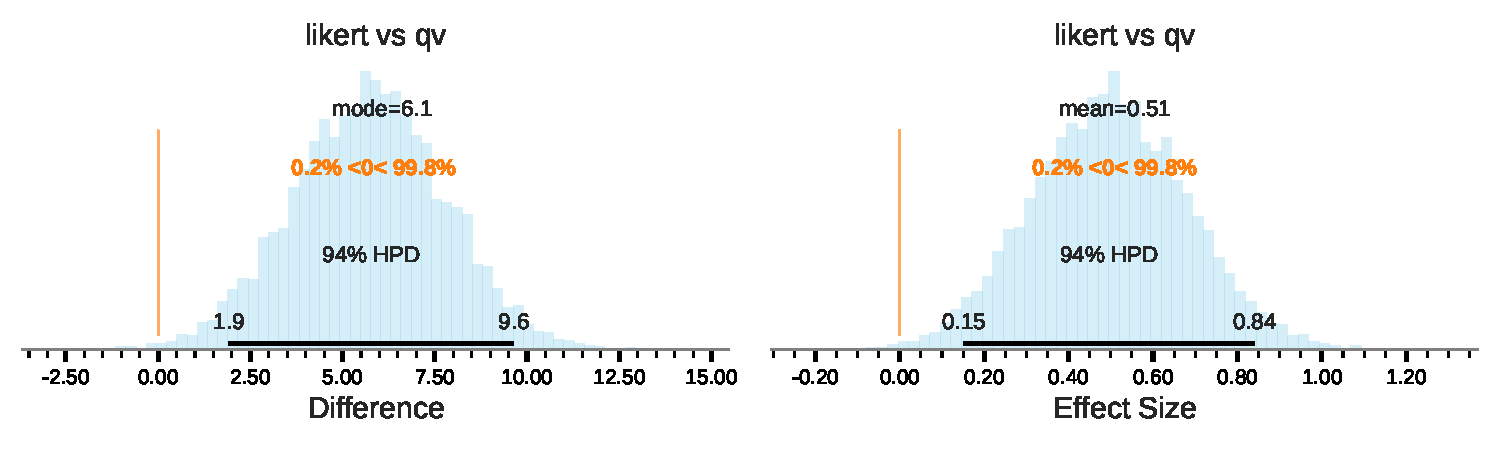
\includegraphics[trim= 0in 0in 0in 0in, clip, width=0.8\textwidth, keepaspectratio=true]{"content/image/Votes_Prices_StudentT_differences_and_effects.pdf"}
  \caption{
    The figure shows the contrasts distribution of the mean cosine similarity angles between the Likert group and QV group. The subgraph on the left shows the absolute difference while the one on the right is about the effect size. Since we are highlighting contrasts, each sub-figure shows an orange vertical line located at 0. \textbf{The main finding is:} survey responses from QV aligned significantly better with the price setting behavior than Likert scale responses with a medium effect size.
  }
  \Description[Contrasts distribution of the mean cosine similarity angles between Likert and QV for experiment two]{Contrasts distribution of the mean cosine similarity angles between Likert and QV for experiment two}
  \label{fig:contrast_exp2}
\end{figure}

Overall, our Bayesian analysis for experiment two showed that QV survey responses aligned significantly better with the price setting behaviors than Likert responses with a medium to high effect size (0.5 - 0.6). The first graph in the left column of~\Cref{fig:traceplot_exp2}, which contains traceplots for the MCMC estimations, shows that the distribution of the mean cosine similarity angle for QV (orange line) is to the left of that for Likert (blue line). Since a perfect alignment means a zero angle, QV had better alignment with the set prices relative to Likert. 

To confirm if the difference was statistical significant, we constructed the distribution of the absolute difference between the means and the distribution of the corresponding effect size (normalized difference), as shown in \Cref{fig:contrast_exp2}. In the subfigure on the left, the mode of the contrast is $6.1$, meaning that the cosine similarity angles in the Likert group were most frequently $6.1$ degrees larger than the angles in the QV group. Since the HPD of [$1.9$, $9.6$] lies outside a significant ROPE (Region of Practical Equivalence) of $0 \pm 1 \deg$, there was a significant difference between the alignment levels of the two survey methods. The medium to high effect size is significant based on the figure on the right, with a modal value of $0.51$ and a HPD interval of [$0.15$, $0.84$].


\begin{sidewaysfigure*}
  \centering
  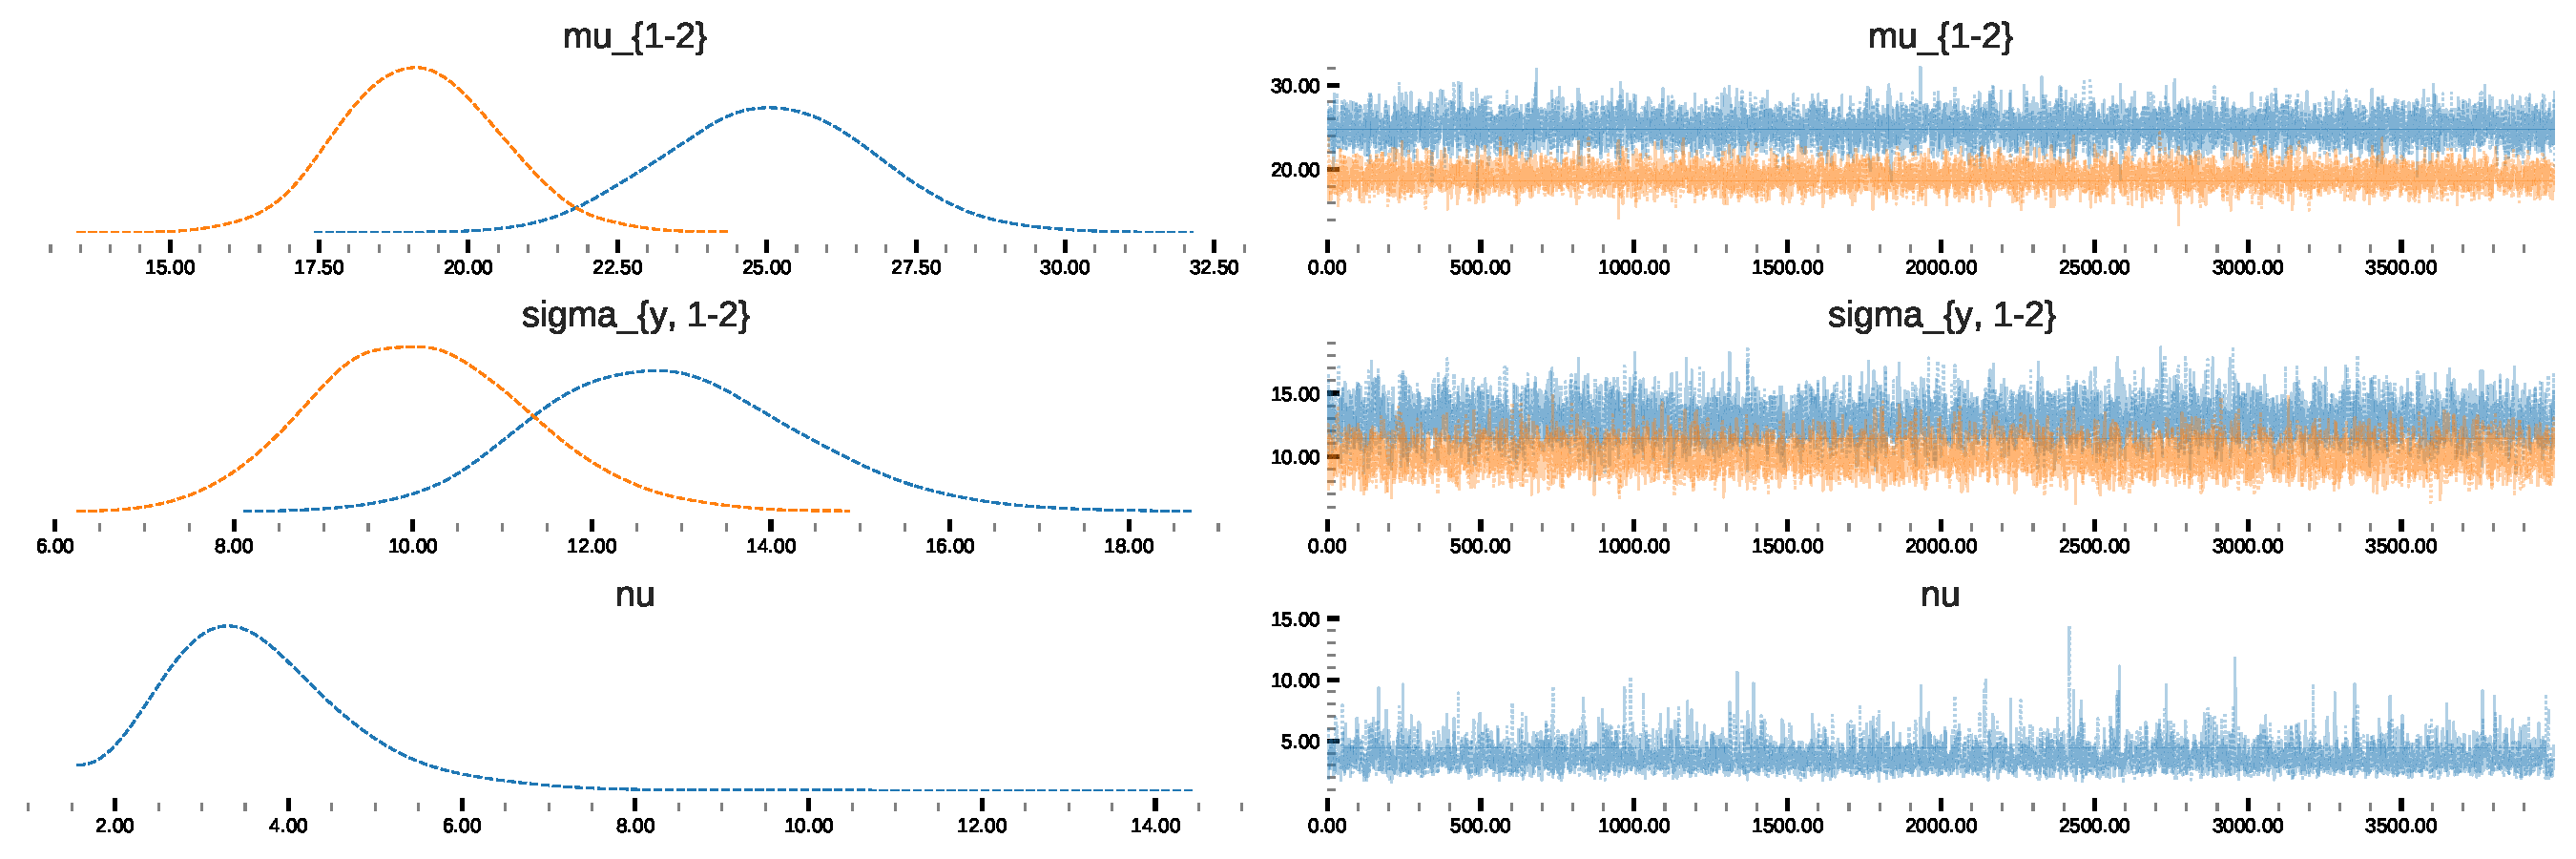
\includegraphics[trim= 0in 0in 0in 0in, clip, width=\textwidth, keepaspectratio=true]{content/image/StudentTIndep_traceplot.pdf}
  \caption{
    Traceplot showing the results of the MCMC estimation in experiment two. The left column is the posterior distributions for $\mu_{1-2}$, $\sigma_{1-2}$, and $\nu$ of the Student-t distribution. The right column shows the corresponding sampling traces. The color mappings are: orange -- QV, blue -- Likert. Distribution for $\mu_{1-2}$ of QV is to the left of Likert, meaning a better alignment with price setting behaviors. Note also, that the modal value for degrees of freedom $\nu \approx 3$, confirming our choice of the Student-t distribution instead of the Normal distribution, which usually requires $\nu \geq 30$. Furthermore, the Gelman-Rubin statistic $\hat{R}$ for all parameters was 1, indicating  convergence of the sampling MCMC chains.
  }
  \Description[Traceplot for the MCMC estimation in experiment two Bayesian model]{Traceplot for the MCMC estimation in experiment two Bayesian model}
  \label{fig:traceplot_exp2}
\end{sidewaysfigure*}
\section{Discussion and Future Work} \label{discussion}
In this section, we discuss implications from the two experiment results. In addition, we lay out intriguing open questions stemmed from this study for future exploration.

\subsection{Does QV Align Better with True Preferences?}
In both RQ1 and RQ2, we ask how well Likert and QV survey results align with people's incentive-compatible behaviors, one in the realm of public policy and the other in HCI research. From the two experiments, we showed that QV aligned significantly better to people's true preferences than Likert surveys in these two areas under the following conditions: (1) the survey question focused on making decisions based on the relative preferences among $K$ options, (2) the $K$ options were either different \textit{aspects} that jointly contributed to the same subject matter or paralleled \textit{options} for the same subject matter, and (3) the QV survey must provide sufficient voice credits ($\geq O(K^{3/2})$, where $K$ is the number of options) to participants. Both experiments showed a significant medium to high effect size for the difference between the degree of alignment in the QV groups and the Likert group. This suggests that QV had the potential to elicit more truthful preferences in collective decision making. We now discuss two potential reasons that may explain the result for RQ1 and RQ2.

\subsubsection{Costs and scarcity}
One explanation for QV's better alignment in the above conditions may be the inherent difference in the notion of costs between QV and Likert when individuals express their opinions. Expressing opinions in Likert does not carry any cost -- an individual could freely select any value, including extreme values, for all $K$ options if one prefer. In QV, participants must pay for their votes for each option at a quadratic cost under a limited budget. 

When costs and a limited budget both exist, participants are facing \textit{scarcity} of resources. In behavioral economics, \textcite{Shah2015a} concluded in their work, ``Scarcity Frames Value'', that individuals would focus on what is really needed and become more rational in decision making under resource constraints. They found that lower-income participants were less susceptible to framing effects than higher-income participants likely because lower-income participants faced stricter resource constraints and thus were better at trade-off thinking. 

In conditions where a survey focuses on understanding how people make trade-offs among $K$ options, as in our two experiments, the concept of scarcity built into the mechanism of QV may help participants make more rational decisions. We observed qualitative supports for this claim from experiment one. [Alternative] After experiencing a drop in the number of voice credits, one participant commented... ""] One participant (\texttt{P24194}), after experiencing a drop in the number of voice credits in the second QV survey, they commented, ``I had fewer credits, so each vote seemed more expensive.'' This comment suggested that participants experienced the idea of ``scarceness'' and resource constraint via the limited voice credit budget during the QV survey.

\subsubsection{Flexibility of expression}
Another potential reason why QV aligned better with incentive-compatible behaviors is a higher degree of flexibility in expressing opinions in QV (with sufficient voice credits) compared to Likert. A five-point Likert survey provides only five choices for each question, which may limit the way a participant can voice their opinion. One Likert group participant in the first experiment (\texttt{P9b3ae}) explicitly mentioned ``[\textellipsis] I would answer otherwise, if there were other options, such as not much, or a little bit.'' Participants wanted to express more fine-grained attitudes while a five-point Likert survey forced them to map their feelings onto a limited fixed scale. QV, in contrast, allows participants to specify the relative distance between two options with greater flexibility, as long as the total cost does not exceed the given credits. The flexibility may enable participants to stay closer to their incentive-compatible preferences and do not need to map to an arbitrary scale.

We compared QV against a five-point Likert scale in this study because the five-point Likert scale is one of the most commonly used Likert scales in various fields \cite{malhotra2006basic}, including public policy and HCI. One may conjecture that a seven-point or eleven-point Likert scale may allow more flexibility than a five-point Likert scale. Debates about the scale format in Likert surveys started in as early as 1965 \cite{komorita1965number}. Some studies found little differences among different scale formats while others did find certain differences \cite{dawes2008data}. We leave the comparison of Likert surveys in other scale formats and QV as an open question to future research.
% This research showed that if the options are homogeneous, a two-point Likert scale yields as high-reliability coefficient as a multi-category system. The research also emphasized that reliability should not be the only metric when deciding which scale is better than the other scale, much more the opposite. It implies that a scale should be chosen for the purpose it aims to serve and the context it is used in. However, in modern research that utilize Likert surveys, there was often little to no discussions describing why the researchers used a specific type of Likert survey. 

\subsection{Effects of the Amount of Voice Credits}
We also investigated how the number of voice credits available to participants impact the QV survey results empirically in part with RQ1. In experiment one, quantitative analysis showed that QV did not elicit more truthful preferences until reaching a sufficient amount of voice credits, as we saw that QV with 36 voice credits ($O(K)$) under-performed QV with 108 ($O(K^{3/2})$) and 324 ($O(K^{2})$) voice credits. We found potential explanations through participants' qualitative responses. 

When participants had only 36 credits in QV, some of them voiced their need to make hard trade-offs. \texttt{P9e5e6} said, ``I think I covered the bare basics.'' and \texttt{Pe37f2} said, ``Less to go around, so had to knuckle down and allocate the most to what I think is most important.'' These responses indicated limited flexibility when the participant's tried expressing their preferences with a small budget.

On the other hand, when given increased voice credits (108 or 324 credits) in their second QV survey, some participants expressed their appreciation for an increased degree of freedom to express their opinions. \texttt{Pcc4aa} reported, ``with more credits I can show what I really like.'' and \texttt{P2d9da} stated, ``Because now that I have a lot more credits, I felt that I could vote on more issues that mean something to me.'' The different qualitative responses for QV36, QV108 and QV324 may not only explain why QV with more voice credits performed better than QV36 in the first experiment, but also lend support to higher level of flexibility being a potential reason for why QV outperformed Likert in the degree of alignment. 

While having fewer voice credits may worsen QV's degree of alignment with participants' incentive-compatible preferences, QV with a stringent budget may be better at eliciting the options participants care the most since it encourages harder trade-offs, based on the qualitative responses above. Future research could explore this potential effect of QV more closely.

In the first experiment, we explored up to a budget of $O(K^{2})$ voice credits, where $K$ is the number of options in the survey, specifically 324 credits. While QV aligned better than Likert up to this amount of voice credits and the percentage of credits used remained high (with a median of 98\%), we suspect that too many voice credits may create excessive cognitive loads to participants. Where the threshold of ``too many'' voice credits lies remains an open question for future work.


\subsection{Open Questions and Future Work}
QV is a relatively new area of research. Comparing the alignment of Likert and QV with user's true preferences is challenging. During the study, we identified various open questions that were yet to address. In this subsection, we propose them as future research directions.

\subsubsection{Comparing ordinal data with numerical data}
To compare ordinal Likert data with numerical donation amounts or set prices, we mapped the five-point Likert scale to integers in the range of $[-2, 2]$. We used the number of votes in QV directly since they are numerical. We made such a decision because selecting "Neutral" (mapped value = 0) in Likert had a similar meaning as casting zero vote in QV.

Whether our approach of mapping Likert data to metric values is the best approach to compare ordinal data with numerical data is debatable. At the same time, identifying the best measure to do so is challenging -- the best way to analyze ordinal Likert data remains a debate till this date \cite{gob2007ordinal}. Future research could explore if there are alternatives to perform such a comparison that circumvents the challenge of mapping ordinal data. 

\subsubsection{Comparing QV with other surveying methods}
% In the previous subsection, we mentioned that Likert survey choices could limit individuals' degree of freedom to express their attitudes. One open question includes investigating if another type of Likert survey influences participants' behavior compared to QV. In addition,
Despite Likert surveys being one of the most-used surveying techniques, we are curious about how other voting mechanisms that involve the concepts of resource constraints or relative-preference elicitation perform compared to QV. Examples include but are not limited to knapsack voting \cite{goel2015knapsack} and ranked-base voting \cite{ledo2018evaluation}. Knapsack voting also uses a budget, but the cost of QV's vote grows quadratically while that of knapsack voting increases linearly. Ranked-based voting focused on eliciting relative rankings among options, which incurs trade-off thinking, but does not show the magnitude of differences between the options, unlike QV. The coexistence of differences and similarities of these voting mechanisms with QV makes the comparison of their performances an interesting open question.

\subsubsection{Upper bound of the number of options}

In our two experiments, the first had 9 options and the second had 5 options on the survey. In both cases, QV performed well, suggesting that participants could make effective trade-offs across up to 9 options. However, our study did not identify the upper bound of the number of options users can handle comfortably on a QV survey. One can imagine the difficulty for QV participants to vote among dozens of survey options. In fact, a work by Iyengar et al. \cite{iyengar2000choice} observed that more choices may not necessarily increase participants' satisfaction, suggesting that people were not good at making choices across an extensive array of options. Therefore, the same question applies in our case -- is there a limit of how many options could be on a QV survey to maintain high-quality data collection?

\subsubsection{Generalizability to different types of surveys}
In this study, we examined QV in two settings. We chose settings that made sense to translate into QV surveys and leveraged prior research. We did not exhaustively examine the type of survey questions that work with QV and those that may not. Hence, readers should take caution in generalizing our results to other types of survey.

In the first experiment, the survey asked participants to choose among $K$ paralleled options for the same subject matter. In the second one, the survey focused on choosing among $K$ aspects that jointly contribute to the same subject matter. The purpose in both surveys were related to relative preferences and trade-offs. We do not yet know if surveys options with other types of relationship would work for QV, e.g., surveys that consist of independent options that do not connect with one another.

Similarly, our study only tested QV in the field of public policy and HCI research. Many other disciplines made use of Likert surveys to make collective decisions. Future research can explore if QV elicits more truthful preferences than Likert in other fields.

\subsubsection{Interface design and mental models}
The final open question is designing a simple, intuitive QV interface for empirical use. QV involves more complicated calculations than Likert. A well-designed interface should reduce a user's cognitive load to help them make accurate decisions easily. Currently, after our iterative-design process, we provided participants information such as the number of votes per option, the voice credits used and remained, and how they allocate the voice credits to each option. 

Different interface designs could nudge users to behave in one specific way instead of another. How the interface should provide voters with these information in an optimal way remains an open question. Understanding individuals' mental models of during voting in QV may inform better designs. Finally, we need to investigate QV interface design for mobile and tablet devices.
% Besides, showing an individual how they had allocated their votes could also potentially interfere and encourage voters to vote for or against an option

\subsection{When to Use QV?}
We showed promising results of QV in our study -- QV elicited more truthful preferences from participants than a five-point Likert scale when making a collective decision to choose among $K$ options. Given the popularity of Likert survey in a wide range of disciplines that involve self-reporting, our research asks an intriguing question of whether there is an alternative survey method that can elicit accurate opinions by leveraging computational power. However, it is critical to reaffirm that the goal of this study is not to claim one survey method should replace another. As aforementioned, there still exist many open questions to understand the nuances in QV. Survey creators should carefully consider the pros and cons (e.g., higher cost to educate participants) of QV and select the best suiting survey method in their contexts.




% \subsection{Where are QV's limitations}
% Experiment two shows a slightly different and more nuanced result.
% It is important to know that
% the characteristics of the ballot options 
% are different compared to experiment one.
% On this ballot, the options are \textit{multiple aspects}
% of a same question.
% In other words, 
% one requires all options 
% to form the result of the final outcome.
% Let us use an analogy:
% If experiment one asks you
% ``how much do you prefer between
% coke, fries, and burgers'',
% the second experiment asks you
% ``how important do you think
% freshness, taste, and texture 
% of your beef patty are?''
% Notice the options in the first question 
% are independent while 
% those in the second question 
% collectively decide how good a beef patty is.

% From an intensity perspective 
% of the aggregated opinions, 
% qualitatively we can observe that 
% the preference result from QV aligns closer 
% to the true preference than that from Likert. 
% We have yet to examine its statistical significance 
% due to an experiment design limitation. 
% From a preference ranking perspective, 
% neither of the results from the Likert survey 
% and QV survey
% diverged significantly 
% from the incentive-compatible behaviors 
% that the buyback group demonstrated. 
% However, part of the Likert results 
% did diverge significantly from the QV results, 
% since aspects in Likert results clustered 
% in the higher rankings, 
% while aspects in the QV results 
% spread out more across the lower rankings. 
% Such finding echoes part of the conclusion 
% in the first experiment, 
% where QV is able to show finer-grained preference results 
% than Likert.

% In conclusion,
% we can conclude that QV with a sufficient budget outperforms Likert surveys when the survey aims to elicit preferences in a 1 in $K$ setting.
% There is not enough statistical evidence yet to conclude whether QV aligns to true preference better than Likert if the survey options are multiple aspects of the same subject. Nevertheless, both experiments demonstrated that QV elicits finer grain preferences from people than Likert in both cases, which is an advantage survey designer could leverage to gain more in-depth understanding of people's opinions.



% \subsection{Design Implications}
% Given these discussions, 
% we propose the following design implications. 
% First, QV provides more fine-grain results,
% including the preference and the level of intensity,
% a group has on a particular topic,
% when deciding among one in $K$ options.
% In the CSCW community,
% we believe this can be applied to 
% many collective decision-making processes.
% Form electing a great project among many,
% to redistributing limited resources among those in need,
% QV serves as an alternative tool 
% than traditional Likert surveys.

\section{Conclusion} \label{conclusion}
In this experiment, we built upon existing empirical literature
and analyzed how QV aligns with participants' true preferences compared with Likert surveys.
We examined the transferability of QV when applied to the HCI domain, and we demonstrated the impact of different voice credits.

\section{Limitation and Future Work} \label{future}

\subsection{Limitation}
We identified two limitations in this study, 
mainly focused on the second experiment.
First, participants in the buyback group
only have one shot.
Some participants did indicate that
they would change what they bought
when they completed the quiz.
It requires further examination
if the first attempt should be considered as one's true preference
or the edited buyback values.

In addition, we are also aware that
designing a between-subject study 
weakened the generalizability 
of the second experiment.
However, we are also aware possible confounds
if both the Likert Group or the QV group completed the buyback.
The buyback will be highly correlated with the survey responses
and it is difficult to issue another task
like in the first experiment
to disconnect participant's cognitive attention
from the video experience, the survey to the buyback.

\subsection{Behavior when casting votes} % slightly boring
It is important to point out that Despite only occurring once (\texttt{P1d659}), we think the term ``voting'' might motivate participants to consider how a collective decision was made.
%scenere voting might not happen in QV?, mentioned in the voting chapter
This participant mentioned ``[\textellipsis] I thought a lot of people would probably support faith and spiritual ecatagory  so I watned to try to counterbalance that by voting against it.'' The participants are willing to pay the cost by devoting fewer votes for issues they care and vote against specific ballots. This behavior is not possible in a Likert survey. This requires further experiments to understand how people's mental model works when voting under QV. \par 

\subsection{Ease of use}
In addition, we do not have enough understanding of the level of usability of QV from two aspects.
First, we are not sure how easy it is for participants to understand QV.
In our experiment, participants are far more familiar with Likert-scaled surveys compared to QV, placing a lighter cognitive load.
We acknowledge that participants need additional time and effort to understand and utilize QV throughout our experiment, yet, it is unclear if education level and prior experiences impact participants' understanding of QV and their final choices.
Second, we do not know if there exists diminished effectiveness of QV if there are large amounts of options, meaning selecting a few over hundreds of options.

\subsection{Interface and medium}
Finally, one crucial unanswered question lies in the medium and interface that QV should be deployed.
It is almost certain that QV will be hard to present on paper since it requires complex calculations. 
Besides, we did not examine if there are differences when voting on a laptop or a handheld device.
We also had not uncovered whether different interface designs, visualization, and additional information impact the performance of QV.


\begin{acks}
Acknowledgments section
\end{acks}

\appendix

\section{Experiment 1 Results}

\subsection{Quantitative Results}
\begin{figure}[htpb]
    \centering
    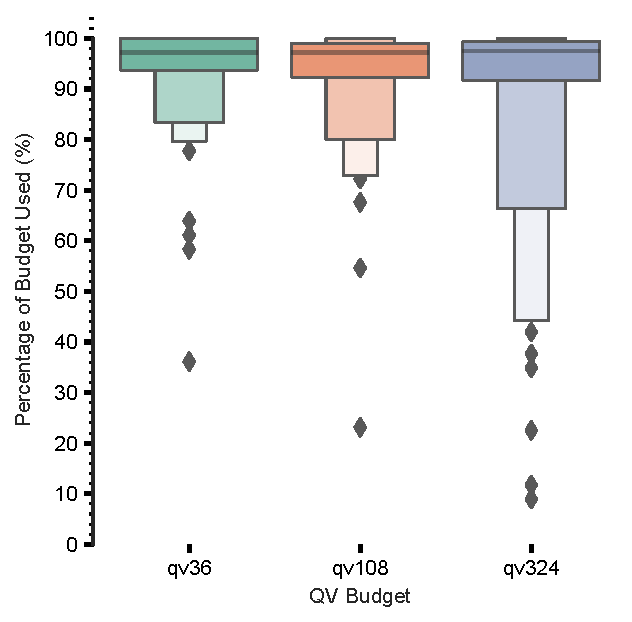
\includegraphics[width=0.5\textwidth, keepaspectratio=true]{content/image/qv_budget_used_distribution.pdf}
    \caption{
      Distribution of Percentage Budget Used in QV36, QV108 and QV324. Percentage budget used is the percentage of voice credits used out of the total voice credits budget available.
    }
    \Description[Distribution of Percentage Budget Used for experiment 1]{Distribution of Percentage Budget Used for experiment 1}
    \label{fig:qv_budget_exp1}
\end{figure}

\subsection{Part Two}

Etiam commodo feugiat nisl pulvinar pellentesque. Etiam auctor sodales
ligula, non varius nibh pulvinar semper. Suspendisse nec lectus non
ipsum convallis congue hendrerit vitae sapien. Donec at laoreet
eros. Vivamus non purus placerat, scelerisque diam eu, cursus
ante. Etiam aliquam tortor auctor efficitur mattis.

\section{Online Resources}

Nam id fermentum dui. Suspendisse sagittis tortor a nulla mollis, in
pulvinar ex pretium. Sed interdum orci quis metus euismod, et sagittis
enim maximus. Vestibulum gravida massa ut felis suscipit
congue. Quisque mattis elit a risus ultrices commodo venenatis eget
dui. Etiam sagittis eleifend elementum.

Nam interdum magna at lectus dignissim, ac dignissim lorem
rhoncus. Maecenas eu arcu ac neque placerat aliquam. Nunc pulvinar
massa et mattis lacinia.

% \bibliography{reference}
% \bibliographystyle{ACM-Reference-Format}
\printbibliography

%\appendix

\section{Experiment 1 Results}

\subsection{Quantitative Results}
\begin{figure}[htpb]
    \centering
    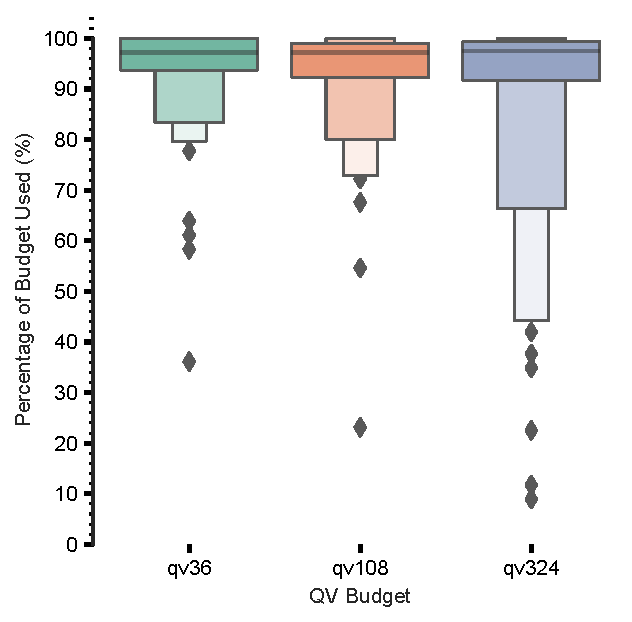
\includegraphics[width=0.5\textwidth, keepaspectratio=true]{content/image/qv_budget_used_distribution.pdf}
    \caption{
      Distribution of Percentage Budget Used in QV36, QV108 and QV324. Percentage budget used is the percentage of voice credits used out of the total voice credits budget available.
    }
    \Description[Distribution of Percentage Budget Used for experiment 1]{Distribution of Percentage Budget Used for experiment 1}
    \label{fig:qv_budget_exp1}
\end{figure}

\subsection{Part Two}

Etiam commodo feugiat nisl pulvinar pellentesque. Etiam auctor sodales
ligula, non varius nibh pulvinar semper. Suspendisse nec lectus non
ipsum convallis congue hendrerit vitae sapien. Donec at laoreet
eros. Vivamus non purus placerat, scelerisque diam eu, cursus
ante. Etiam aliquam tortor auctor efficitur mattis.

\section{Online Resources}

Nam id fermentum dui. Suspendisse sagittis tortor a nulla mollis, in
pulvinar ex pretium. Sed interdum orci quis metus euismod, et sagittis
enim maximus. Vestibulum gravida massa ut felis suscipit
congue. Quisque mattis elit a risus ultrices commodo venenatis eget
dui. Etiam sagittis eleifend elementum.

Nam interdum magna at lectus dignissim, ac dignissim lorem
rhoncus. Maecenas eu arcu ac neque placerat aliquam. Nunc pulvinar
massa et mattis lacinia.

\end{document}
\endinput

